\documentclass[UTF8,a4paper,12pt]{ctexart}

% ===================== 基本宏包 =====================
\usepackage{amsmath,amssymb}
\usepackage{geometry}
\usepackage{graphicx}
\usepackage{booktabs}
\usepackage{longtable}
\usepackage{float}
\usepackage{hyperref}
\usepackage{array}
\usepackage{xcolor}
\usepackage{tikz}
\usepackage{setspace}
\usepackage{fontspec}
\usepackage{fancyhdr}
\usepackage{enumitem}
\usepackage{caption}
\usepackage{indentfirst}
\usetikzlibrary{arrows.meta,positioning}

% ===================== 页面设置 =====================
\geometry{left=2.5cm,right=2.5cm,top=2.5cm,bottom=2.5cm}
\graphicspath{{figures/}}

% ===================== 字体设置 =====================
% 编译方式必须使用 XeLaTeX
% 正文中文：宋体；英文和数字：Times New Roman
\setmainfont{Times New Roman}
\setCJKmainfont[AutoFakeBold=3]{SimSun}

% ===================== 正文格式 =====================
% 小四宋体，1.5 倍行距，首行缩进 2 字符
\AtBeginDocument{\zihao{-4}\songti}
\onehalfspacing
\setlength{\parindent}{2em}

% ===================== 标题格式设置 =====================
% 一级、二级、三级标题：小四，黑体，相当于中文加粗效果
\ctexset{
	section = {
		format = {\zihao{-4}\heiti},
		name = {},
		number = \arabic{section},
		aftername = \quad,
		beforeskip = 1.5ex,
		afterskip = 1.0ex
	},
	subsection = {
		format = {\zihao{-4}\heiti},
		name = {},
		number = \thesection.\arabic{subsection},
		aftername = \quad,
		beforeskip = 1.2ex,
		afterskip = 0.8ex
	},
	subsubsection = {
		format = {\zihao{-4}\heiti},
		name = {},
		number = \thesubsection.\arabic{subsubsection},
		aftername = \quad,
		beforeskip = 1.0ex,
		afterskip = 0.6ex
	}
}

% ===================== 图表标题设置 =====================
% 图表 caption：小五，加粗，居中
\DeclareCaptionFont{xiaowu}{\zihao{-5}\heiti}
\captionsetup{
	font=xiaowu,
	labelfont=xiaowu,
	labelsep=space,
	justification=centering
}

% ===================== 页眉页脚设置 =====================
% 页码放在每页正下方中间
\pagestyle{fancy}
\fancyhf{}
\fancyfoot[C]{\thepage}
\renewcommand{\headrulewidth}{0pt}
\renewcommand{\footrulewidth}{0pt}

\fancypagestyle{plain}{
	\fancyhf{}
	\fancyfoot[C]{\thepage}
	\renewcommand{\headrulewidth}{0pt}
	\renewcommand{\footrulewidth}{0pt}
}

% ===================== 超链接设置 =====================
\hypersetup{
	colorlinks=true,
	linkcolor=black,
	citecolor=black,
	urlcolor=blue
}

% ===================== 文档开始 =====================
\begin{document}
	
	% ===================== 封面 =====================
	\begin{titlepage}
		\thispagestyle{empty}
		\centering
		
		\begin{figure}[h!]
			
\includegraphics[width=\textwidth]{pic.png}
		\end{figure}
		
		\vspace*{1cm}
		
		{\zihao{1}\heiti \textbf{多机械臂搬运调度与模式选择}\par}
		
		\vspace{0.5cm}
		
		{\zihao{3}\heiti 运筹学课程大作业\par}
		
		\vspace{1.5cm}
		
		\renewcommand{\arraystretch}{1.8}
		{\zihao{-4}\songti
			\begin{tabular}{>{\heiti}r p{8cm}}
				团队成员： & \underline{\makebox[8cm][c]{修嘉卿3240104703}} \\[0.4cm]
					& \underline{\makebox[8cm][c]{
							傅安澜3240104374}} \\[0.4cm]
						& \underline{\makebox[8cm][c]{王沐灵3240101575}} \\[0.4cm]
				专业：     & \underline{\makebox[8cm][c]{自动化（电气学院）}} \\[0.4cm]
				指导老师： & \underline{\makebox[8cm][c]{何衍}} \\[0.4cm]
				日期：     & \underline{\makebox[8cm][c]{\today}} \\
			\end{tabular}
		}
		
		\vfill
	\end{titlepage}
	
	% ===================== 目录 =====================
	\pagenumbering{arabic}
	\tableofcontents
	\newpage
	
	% ===================== 正文 =====================
	
\section*{摘要}
\addcontentsline{toc}{section}{摘要:}

本文围绕多机械臂搬运场景中的任务调度与运行模式选择问题展开研究。针对圆形作业区域内多类待搬运物块、不同类型收集盒以及双臂协同搬运需求，本文将实际机械臂搬运过程抽象为一个具有任务分配、执行排序、资源互斥和协同约束的运筹学优化问题。研究对象不是机械臂的底层运动控制或动力学建模，而是在给定任务、机械臂数量、作业时间和能耗参数的条件下，合理安排每个物块的执行机械臂、搬运顺序和协同模式，使系统整体完成时间较短、能耗较低，并兼顾机械臂之间的负载均衡。

在模型构建方面，本文以物块搬运任务为基本调度单元，考虑单臂搬运任务与双臂协同搬运任务的差异，建立了包含任务选择变量、开始时间变量、完成时间变量和模式选择变量的整数规划模型。目标函数以最小化最大完成时间为主，同时引入能耗指标和负载均衡指标用于评价不同调度方案的综合性能。针对该问题的组合复杂性，本文设计并实现了四类求解方法，包括 CP-SAT 求解器、融合剪枝的隐枚举法、启发式算法以及热启动后的隐枚举法，并通过多组算例对不同方法的求解效果和计算效率进行了比较。

在此基础上，本文进一步引入非线性优化分析，对机械臂速度倍率与时间、能耗之间的关系进行建模，研究不同速度选择对搬运效率和能耗代价的影响。同时，本文结合 KKT 条件对非线性优化结果进行可行性和最优性验证，并通过二臂与三臂场景的对比分析，讨论增加机械臂数量后系统在完成时间、能耗和模式选择方面的变化规律。实验结果表明，融合剪枝的隐枚举法能够在保持较高求解质量的同时减少无效搜索，启发式算法具有较好的计算速度，热启动后的隐枚举法能够进一步利用已有可行解提高搜索效率；非线性优化部分则说明机械臂速度调整会带来时间收益与能耗代价之间的权衡，为多机械臂调度方案的综合评价提供了补充依据。


\noindent {\heiti 关键词：}
多机械臂调度；运筹学优化；整数规划；隐枚举法；分支定界；启发式算法；非线性优化；KKT 条件
	\section{前言}

\subsection{研究背景}

随着自动化技术和智能制造系统的发展，多机械臂协同作业逐渐成为仓储搬运、工业分拣、柔性装配和物流输送等场景中的重要研究方向。与单机械臂系统相比，多机械臂系统具有更强的并行作业能力，能够在同一作业区域内同时完成多个搬运任务，从而缩短整体作业时间，提高系统运行效率。然而，多机械臂系统也带来了更加复杂的调度问题：不同机械臂之间可能存在空间资源冲突，部分任务需要两只机械臂协同完成，不同任务之间存在执行顺序差异，同时系统还需要在完成时间、能耗和资源利用率之间进行综合权衡。

在实际搬运场景中，待搬运物块通常具有不同的尺寸、重量和目标位置。较小或较轻的物块可以由单只机械臂独立搬运，而较大或较重的物块则需要两只机械臂协同完成。与此同时，不同类别的物块需要被搬运到不同的收集盒中，任务的空间位置、搬运距离和协同要求都会影响最终调度结果。因此，多机械臂搬运问题并不是简单的任务平均分配问题，而是一个同时涉及任务分配、执行排序、资源互斥、协同模式选择和目标优化的组合优化问题。

运筹学中的整数规划、调度优化、分支定界和启发式算法为该类问题提供了有效的建模与求解工具。通过将机械臂视为有限作业资源，将物块搬运过程视为一组具有时间和资源约束的任务，可以把实际搬运问题转化为可求解的数学优化模型。在此基础上，结合精确求解算法与自定义搜索策略，不仅可以获得较优调度方案，还可以分析不同算法在求解质量、计算时间和适用场景方面的差异。

\subsection{研究现状}

现有多机械臂协同作业研究大多可以分为两个方向。一类研究侧重于机器人学层面的运动规划、轨迹控制、避障控制和动力学协调，重点解决机械臂如何稳定、准确地完成运动的问题；另一类研究则侧重于系统调度和任务规划，重点关注在多个任务和多个执行资源之间如何进行分配和排序。本文关注的是后者，即从运筹学角度研究多机械臂搬运任务的调度优化问题，而不涉及机械臂底层关节轨迹、运动学逆解和动力学控制。

在调度优化方法方面，整数规划模型能够较完整地描述任务选择、资源占用和时间先后关系，适合用于构建标准化数学模型。CP-SAT 求解器等通用优化工具能够对中小规模问题给出较高质量的解，但在问题规模增大或约束复杂时，求解时间可能明显增加。隐枚举法和分支定界思想则适合处理具有离散决策结构的问题，通过逐步构造候选解并利用当前最优上界、可行性判断和下界估计提前剪枝，可以避免对所有组合方案进行完全枚举。启发式算法虽然通常不能保证全局最优，但具有实现简单、计算速度快和适合快速生成可行解的特点，在实际工程问题中也具有较强应用价值。

对于多机械臂搬运任务而言，仅比较调度完成时间并不足以全面评价方案优劣。若机械臂通过提高运行速度来缩短搬运时间，往往会导致能耗增加；若增加机械臂数量，虽然可能提升并行搬运能力，但也可能带来额外的启用成本和能耗代价。因此，在基础整数规划模型之外，引入非线性速度--能耗分析，有助于进一步说明调度方案背后的时间收益与能耗代价之间的关系。

\subsection{研究意义}

本文研究的意义主要体现在三个方面。

首先，从实际问题抽象角度看，本文将多机械臂搬运场景转化为运筹学中的调度优化问题，明确区分了机械臂底层控制问题与任务层调度问题。通过设置任务分配变量、时间变量和模式选择变量，可以较清晰地描述单臂搬运、双臂协同搬运、多类别收集盒以及机械臂资源互斥等实际约束，使问题具有明确的数学表达。

其次，从算法设计角度看，本文不仅使用 CP-SAT 求解器作为标准优化工具，还设计了融合剪枝的隐枚举法、启发式算法和热启动后的隐枚举法。不同方法之间既有精确求解与近似求解的对比，也有通用求解器与自定义算法的对比。通过比较各方法在不同任务规模和不同场景下的运行结果，可以分析剪枝策略、启发式规则和热启动机制对求解效率的影响。

最后，从结果分析角度看，本文不仅关注最终调度方案是否可行，还进一步比较二臂与三臂场景下的完成时间、能耗和综合表现，并通过非线性优化分析讨论速度调整带来的时间--能耗权衡。这样的分析能够说明多机械臂系统并不是机械臂数量越多越好，也不是运行速度越快越优，而是需要根据任务规模、物块类型、协同需求和能耗约束进行综合判断。

\subsection{本文主要内容}

本文的主要研究内容如下。

第一，建立多机械臂搬运调度优化模型。根据多类别物块、不同目标收集盒、单臂与双臂协同搬运模式等实际条件，构建包含任务分配、时间一致性、资源互斥和序列转移约束的数学模型，并给出相应目标函数。

第二，设计并实现多种求解方法。本文分别采用 CP-SAT 求解器、融合剪枝的隐枚举法、启发式算法以及热启动后的隐枚举法进行求解，并从算法思想、实现方式和适用特点等角度进行说明。

第三，开展算例分析与方法对比。通过多组不同任务规模和不同机械臂数量的算例，比较各方法得到的最大完成时间、能耗、运行时间和负载均衡效果，分析不同算法的优缺点。

第四，进行非线性速度--能耗优化分析。在基础调度结果上，引入速度倍率变量，建立速度与作业时间、能耗之间的非线性关系，并结合 KKT 条件对优化结果进行验证，进一步讨论二臂与三臂模式选择中的时间收益和能耗代价。
	\section{问题描述}

本项目关注的是\textbf{多机械臂搬运任务的运筹学调度求解与二臂/三臂运行模式选择}，不是机器人运动学、动力学建模或轨迹控制问题；机械臂在本文中主要作为\textbf{可分配的作业资源}参与调度优化。

因此，本文并不研究机械臂关节角、末端轨迹、动力学方程或控制器设计，而是将多机械臂搬运过程抽象为一个具有\textbf{任务分配、执行排序、资源互斥、安全区占用和多目标优化}特征的调度问题。本章主要回答三个问题：第一，实际搬运任务如何抽象为任务集合与执行模式；第二，时间、能耗和安全约束如何用数学符号表达；第三，如何建立同时考虑\textbf{最大完工时间、总能耗和负载均衡}的优化模型。

\subsection{问题场景}

考虑一个圆形作业区域，区域中随机放置若干待搬运方块。每个方块具有类型、重量、初始位置和目标收集盒。系统中可配置两只或三只机械臂，机械臂从各自的待机位置出发，将方块搬运到对应类型的收集盒中。四类方块的任务属性如下：

\begin{table}[H]
    \centering
    \caption{方块类型与任务属性}
    \begin{tabular}{ccccc}
        \toprule
        方块类型 & 任务类型 & 所需机械臂数 & 目标收集盒 & 相对搬运难度 \\
        \midrule
        Type1 & 单臂任务 & 1 & Box1 & 小而轻 \\
        Type2 & 单臂任务 & 1 & Box2 & 小但较重 \\
        Type3 & 双臂协同任务 & 2 & Box3 & 大且需协同 \\
        Type4 & 双臂协同任务 & 2 & Box4 & 大且较重，协同代价高 \\
        \bottomrule
    \end{tabular}
    \label{tab:block_type_task}
\end{table}

图 \ref{fig:workspace_example} 给出同一组任务实例在两臂系统和三臂系统下的工作空间示意。图中蓝色圆形区域表示方块随机生成的作业区域，橙色虚线圆表示中心安全参考区，方形标记表示机械臂基座，菱形标记表示四类收集盒，圆点表示待搬运方块，虚线表示方块到对应收集盒的搬运方向。方块旁标注的机械臂组合为该案例求解得到的任务分配结果。

\begin{figure}[H]
    \centering
    \begin{minipage}{0.48\textwidth}
        \centering
        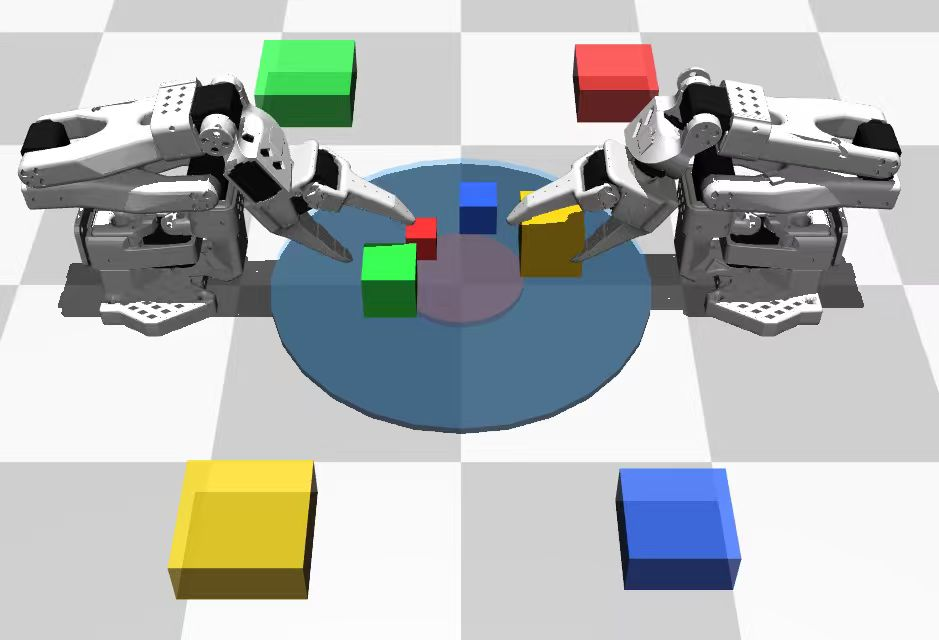
\includegraphics[width=\linewidth]{workspace_two_arm_example.jpg}
        \par\small (a) 两臂系统示意
    \end{minipage}
    \hfill
    \begin{minipage}{0.48\textwidth}
        \centering
        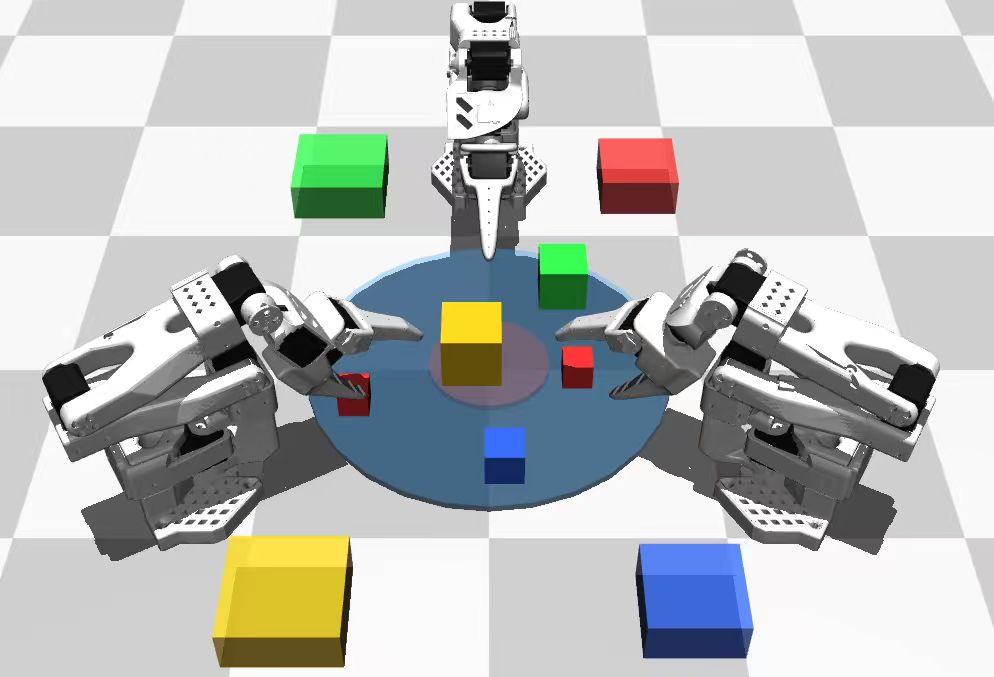
\includegraphics[width=\linewidth]{workspace_three_arm_example.jpg}
        \par\small (b) 三臂系统示意
    \end{minipage}
    \caption{多机械臂分类搬运任务的工作空间示意}
    \label{fig:workspace_example}
\end{figure}

在两臂系统中，双臂协同任务只能由两只机械臂共同完成；在三臂系统中，双臂协同任务可以从三只机械臂中选择任意两只共同完成。因此，三臂系统一方面增加了\textbf{可选执行模式和并行能力}，可能缩短最大完工时间；另一方面也会带来额外的系统固定能耗和协同协调代价。本文后续案例分析正是围绕这一\textbf{时间--能耗权衡}展开。

此外，作业区域中心附近设置安全区。当某个任务的搬运路径经过中心安全区时，该任务组需要占用中心区资源。这里的中心区不是单只机械臂层面的互斥资源，而是任务组层面的共享安全资源：同一个双臂协同任务内部的两只机械臂允许同时进入中心区，但不同任务组不能同时占用中心区。

\subsection{集合、参数与执行模式}

设任务集合为
\[
    \mathcal{J}=\{1,2,\ldots,n\}.
\]
两臂系统和三臂系统的机械臂集合分别为
\[
    \mathcal{A}^{(2)}=\{\mathrm{arm1},\mathrm{arm2}\},\qquad
    \mathcal{A}^{(3)}=\{\mathrm{arm1},\mathrm{arm2},\mathrm{arm3}\}.
\]
下文若不特别区分两臂或三臂，统一记机械臂集合为 $\mathcal{A}$，其规模为
$|\mathcal{A}|=m$，其中 $m\in\{2,3\}$。

每个任务 $j\in\mathcal{J}$ 对应一个方块。为便于后续建模，表 \ref{tab:basic_symbols} 汇总主要任务参数。

\begin{table}[H]
    \centering
    \caption{任务与系统参数说明}
    \begin{tabular}{c >{\centering\arraybackslash}p{0.68\textwidth}}
        \toprule
        符号 & 含义 \\
        \midrule
        $p_j$ & 任务 $j$ 对应方块的初始位置 \\
        $q_j$ & 任务 $j$ 对应目标收集盒的位置 \\
        $b_j$ & 方块类型，$b_j\in\{1,2,3,4\}$ \\
        $r_j$ & 完成任务 $j$ 所需机械臂数量 \\
        $w_j$ & 方块重量 \\
        $d_j$ & 方块从初始位置到目标收集盒的搬运距离 \\
        \bottomrule
    \end{tabular}
    \label{tab:basic_symbols}
\end{table}

不同方块类型决定任务所需机械臂数量：
\[
    r_j=
    \begin{cases}
    1, & b_j\in\{1,2\},\\
    2, & b_j\in\{3,4\}.
    \end{cases}
\]
搬运距离定义为
\[
    d_j=\|p_j-q_j\|_2.
\]

对每个任务 $j$，根据可达性和所需机械臂数构造可行执行模式集合 $\mathcal{M}_j$。一个执行模式 $k\in\mathcal{M}_j$ 包含以下信息：
\[
    k=(j,A_k,t_k,e_k,z_k),
\]
其含义如表 \ref{tab:mode_symbol} 所示。

\begin{table}[H]
    \centering
    \caption{执行模式 $k$ 的组成}
    \begin{tabular}{c >{\centering\arraybackslash}p{0.68\textwidth}}
        \toprule
        符号 & 含义 \\
        \midrule
        $j$ & 该模式对应的任务编号 \\
        $A_k$ & 执行该模式占用的机械臂集合，满足 $A_k\subseteq\mathcal{A}$ 且 $|A_k|=r_j$ \\
        $t_k$ & 该模式下的任务处理时间 \\
        $e_k$ & 该模式下的任务处理能耗 \\
        $z_k$ & 是否经过中心安全区，$z_k=1$ 表示经过，$z_k=0$ 表示不经过 \\
        \bottomrule
    \end{tabular}
    \label{tab:mode_symbol}
\end{table}

\subsubsection{任务处理时间}

本文将机械臂完成一个任务的时间分为两部分：一是执行当前任务本身所需的处理时间，二是任务之间的空载转移时间。这里先定义任务处理时间；空载转移时间将在后续序列相关约束中单独建模。

任务处理时间只描述机械臂到达方块位置后，将方块搬运到目标收集盒所需的时间。它由负载搬运时间、抓取/放置服务时间和安全缓冲时间组成。设单臂负载速度为 $v_s$，双臂协同负载速度为 $v_d$，则
\[
    t_k=
    \begin{cases}
    \left(d_j/v_s+T_s+T_{\mathrm{safe}}\right)\cdot \kappa_t, & |A_k|=1,\\
    \left(d_j/v_d+T_d+T_{\mathrm{safe}}\right)\cdot \kappa_t, & |A_k|=2,
    \end{cases}
\]
其中 $d_j/v_s$ 或 $d_j/v_d$ 表示带负载搬运阶段的行走时间；$T_s,T_d$ 分别表示单臂和双臂任务的抓取、夹持稳定与放置服务时间；$T_{\mathrm{safe}}$ 为调度层面的等效安全缓冲时间，用于表示对准、同步、放置稳定等未单独细分的短时间余量。$\kappa_t$ 为时间离散化尺度，代码实现中取 $\kappa_t=100$，即将 1 秒连续时间转换为 100 个整数 tick，以便整数规划和分枝定界算法处理。

\subsubsection{任务处理能耗}

任务处理能耗采用等效能耗模型描述，用于在调度层面区分不同方块类型的搬运难度。该能耗并不是对电机电流、关节力矩等底层物理量的精确预测，而是根据方块重量、搬运距离、任务持续时间和双臂协同复杂度构造的综合评价指标。这里定义的处理能耗记为 $e_k$，即后文系统总能耗公式中 $\sum e_kx_k$ 对应的任务执行能耗项。

对任务 $j$ 的某个执行模式 $k$，其处理能耗可表示为
\[
    e_k=\kappa_e\left(
    \phi_j E_{jk}^{\mathrm{load}}
    +E_{jk}^{\mathrm{grasp}}
    +|A_k|h_j\frac{t_k}{\kappa_t}
    +\sigma_j\eta_m
    \right).
\]
其中，$E_{jk}^{\mathrm{load}}$ 为基础负载搬运能耗，与方块重量和搬运距离有关；$E_{jk}^{\mathrm{grasp}}$ 为抓取、夹持建立和放置动作产生的服务能耗；$|A_k|h_jt_k/\kappa_t$ 表示任务执行期间参与机械臂维持夹持与稳定搬运所需的保持能耗；$\sigma_j\eta_m$ 表示双臂协同任务中的额外同步协调代价及系统规模修正。$\kappa_e$ 为能耗离散化尺度，用于将连续能耗转换为整数能耗值，以便与整数规划和分支定界算法统一。

为刻画不同方块类型对能耗的影响，引入表 \ref{tab:energy_type_params} 中的类型相关参数。

\begin{table}[H]
    \centering
    \caption{方块类型相关能耗参数}
    \begin{tabular}{
        >{\centering\arraybackslash}p{0.18\textwidth}
        >{\centering\arraybackslash}p{0.24\textwidth}
        >{\centering\arraybackslash}p{0.46\textwidth}
    }
        \toprule
        参数 & 名称 & 含义 \\
        \midrule
        $\phi_j$ & 载荷修正系数 & 放大搬运难度对能耗的影响 \\
        $h_j$ & 保持功率 & 单位时间内的夹持与稳定搬运代价 \\
        $\sigma_j$ & 同步能耗 & 双臂协同任务的一次性协调代价 \\
        \bottomrule
    \end{tabular}
    \label{tab:energy_type_params}
\end{table}

对于 Type1 和 Type2 单臂任务，任务不涉及双臂同步，因此令 $\sigma_j=0$，且 $|A_k|=1$。对于 Type3 和 Type4 双臂协同任务，$\sigma_j$ 取正值，$|A_k|=2$，用于刻画两只机械臂在同步支撑、同步移动和协调放置过程中的额外能耗。两臂系统中 $\eta_m=1$；三臂系统虽然每个双臂任务仍只使用两只机械臂，但可选组合更多、调度协调更复杂，因此 $\eta_m$ 可取略大于 1 的值。其中 Type4 方块的搬运难度更高，因此其 $\phi_j$、$h_j$ 或 $\sigma_j$ 可设置为更大的取值。

\subsection{决策变量}

为了同时描述任务模式选择、时间安排和机械臂作业顺序，定义如下决策变量。

\begin{itemize}
    \item $x_k\in\{0,1\}$：若任务执行模式 $k$ 被选择，则 $x_k=1$，否则为 0。
    \item $S_k,E_k$：模式 $k$ 对应任务处理段的开始时间和结束时间。
    \item $y_{a,u,v}\in\{0,1\}$：对机械臂 $a$，若其作业顺序中模式 $u$ 后紧接模式 $v$，则 $y_{a,u,v}=1$。虚拟模式 $0$ 表示机械臂的待机位置，因此 $y_{a,0,v}=1$ 表示 $v$ 是机械臂 $a$ 的首个任务，$y_{a,u,0}=1$ 表示 $u$ 是其末个任务。
    \item $C_{\max}$：所有任务的最大完工时间。
    \item $E_{\mathrm{tot}}$：系统总能耗。
    \item $L_a$：机械臂 $a$ 的总负载时间，包括任务处理时间和空载转移时间。
    \item $B$：机械臂负载不均衡度，即最大负载与最小负载之差。
\end{itemize}

其中，$y_{a,u,v}$ 用于描述序列相关 setup。机械臂执行完一个任务后，需要从上一任务目标收集盒移动到下一任务的方块初始位置；若该任务是该机械臂的第一个任务，则需要从机械臂待机位置移动到该方块位置。这部分空载转移时间和能耗都与任务顺序有关。为简化后续公式，定义参数
\[
    \delta_{a,k}=\begin{cases}
    1, & a\in A_k,\\
    0, & a\notin A_k,
    \end{cases}
    \qquad
    \mathcal M_a=\{k:\delta_{a,k}=1\}.
\]

\subsection{约束条件}
\begin{enumerate}
\item \textbf{任务唯一执行模式约束}

每个任务必须且只能选择一种可行执行模式：
\[
    \sum_{k\in\mathcal{M}_j}x_k=1,\quad \forall j\in\mathcal{J}.
\]
该约束保证每个方块都被搬运一次，且不会被多个模式重复执行。

\item \textbf{时间一致性约束}

若模式 $k$ 被选择，则其结束时间等于开始时间加处理时间：
\[
    E_k=S_k+t_k,\quad \forall k \text{ with } x_k=1.
\]
在整数规划实现中，未被选择的模式通过可选区间变量处理；在自编算法中，未被选择的模式不会进入调度序列。

\item \textbf{机械臂资源互斥约束}

同一只机械臂在同一时刻不能执行两个任务。若两个被选择模式 $u,v$ 均占用机械臂 $a$，则必须满足二者在时间轴上不重叠：
\[
    [S_u,E_u)\cap [S_v,E_v)=\varnothing,\quad
    \forall a\in A_u\cap A_v.
\]
基础模型中该约束通过 NoOverlap 资源约束实现；自编求解器中则通过维护每只机械臂的可用时间递推生成可行调度。

\item \textbf{序列相关空载转移约束}

首先需要使顺序变量与模式选择变量一致。对每只机械臂，任一被选模式恰有一个前驱和一个后继：
\[
    \sum_{\substack{u\in\mathcal M_a\cup\{0\}\\u\ne v}}y_{a,u,v}
    =\delta_{a,v}x_v,
    \qquad \forall a\in\mathcal A,\ v\in\mathcal M_a,
\]
\[
    \sum_{\substack{v\in\mathcal M_a\cup\{0\}\\v\ne u}}y_{a,u,v}
    =\delta_{a,u}x_u,
    \qquad \forall a\in\mathcal A,\ u\in\mathcal M_a.
\]
同时令虚拟节点 $0$ 具有至多一条出弧和一条入弧，并施加单回路约束以消除不经过虚拟节点的子回路。代码中上述关系由 \texttt{AddCircuit} 统一实现；当机械臂未承担任务时，采用虚拟自环 $(0,0)$。

设机械臂 $a$ 执行完模式 $u$ 后紧接执行模式 $v$，则模式 $v$ 的开始时间必须不早于模式 $u$ 的结束时间加空载转移时间：
\[
    S_v\ge E_u+\tau_{u,v},\quad \text{if } y_{a,u,v}=1,
    \qquad u,v\in\mathcal M_a.
\]
其中
\[
    \tau_{u,v}=\frac{\|q_u-p_v\|_2}{v_0}\cdot \kappa_t,
\]
$v_0$ 为空载移动速度。若 $v$ 是机械臂 $a$ 的第一个任务，则
\[
    S_v\ge \tau^a_{0,v}
    =\frac{\|o_a-p_v\|_2}{v_0}\cdot \kappa_t,
    \quad \text{if }y_{a,0,v}=1,
\]
其中 $o_a$ 为机械臂 $a$ 的待机位置。

相应的空载转移能耗记为
\[
    \epsilon_{u,v}=\alpha_0\|q_u-p_v\|_2\cdot \kappa_e,
    \qquad
    \epsilon^a_{0,v}=\alpha_0\|o_a-p_v\|_2\cdot \kappa_e,
\]
首任务从待机位置出发时同理计算。该项将计入系统总能耗。

\item 中心安全区互斥约束

参数 $z_k\in\{0,1\}$ 表示模式 $k$ 的负载搬运路径是否经过中心安全区。对于两个不同任务的已选模式 $u,v$，若 $z_u=z_v=1$，则其中心区占用时间不能重叠：
\[
    [S_u,E_u)\cap [S_v,E_v)=\varnothing,
    \quad \text{if }x_u=x_v=z_u=z_v=1,
    \quad j(u)\ne j(v).
\]
该约束体现中心安全区在任务组层面的互斥。需要强调的是，对于同一个双臂协同任务，其内部两只机械臂属于同一任务组，不构成彼此冲突。

\item 最大完工时间、总能耗与负载均衡约束

最大完工时间满足
\[
    C_{\max}\ge E_k,\quad \forall k \text{ with } x_k=1.
\]

系统总能耗由处理能耗、空载转移能耗和系统级固定开销组成：
\[
    E_{\mathrm{tot}}
    =
    \sum_{j\in\mathcal{J}}\sum_{k\in\mathcal{M}_j}e_kx_k
    +\sum_{a\in\mathcal{A}}\sum_{\substack{u,v\in\mathcal M_a\\u\ne v}}
    \epsilon_{u,v}y_{a,u,v}
    +\sum_{a\in\mathcal A}\sum_{v\in\mathcal M_a}
    \epsilon^a_{0,v}y_{a,0,v}
    +mE_{\mathrm{sys}},
\]
其中 $E_{\mathrm{sys}}$ 为单只机械臂的启动、上电、伺服保持和控制通信等效固定能耗。

机械臂负载 $L_a$ 包括该机械臂承担的处理时间和空载转移时间：
\[
    L_a=
    \sum_k\delta_{a,k}t_kx_k
    +\sum_{\substack{u,v\in\mathcal M_a\\u\ne v}}\tau_{u,v}y_{a,u,v}
    +\sum_{v\in\mathcal M_a}\tau^a_{0,v}y_{a,0,v}.
\]
负载均衡指标定义为
\[
    B=\max_{a\in\mathcal{A}}L_a-\min_{a\in\mathcal{A}}L_a.
\]
\end{enumerate}

\subsection{目标规划模型}

本问题同时关注完成效率、运行能耗和机械臂利用均衡，三个目标按时间、能耗、负载均衡的顺序具有严格优先级。统一目标框架为
\[
    \operatorname{lexmin}\bigl(C_{\max},E_{\mathrm{tot}},B\bigr).
\]
其具体含义为：
\[
    P_1:\quad \min C_{\max},
\]
\[
    P_2:\quad \min E_{\mathrm{tot}},
    \qquad \text{s.t. }C_{\max}=C_{\max}^{\star},
\]
\[
    P_3:\quad \min B,
    \qquad \text{s.t. }C_{\max}=C_{\max}^{\star},\quad
    E_{\mathrm{tot}}=E_{\mathrm{tot}}^{\star}.
\]
即先保证整体任务尽快完成，再在不牺牲时间目标的前提下降低能耗，最后改善机械臂负载均衡。各求解方法遵循相同的优先级，但实现形式不同。

\subsubsection{CP-SAT 的偏差变量目标规划形式}

基础 CP-SAT 方法采用带偏差变量的目标规划。设 $G_T,G_E,G_B$ 为三个理想目标值，引入非负偏差变量 $d_i^+,d_i^-$：
\[
\begin{aligned}
    C_{\max}+d_1^- -d_1^+ &=G_T,\\
    E_{\mathrm{tot}}+d_2^- -d_2^+ &=G_E,\\
    B+d_3^- -d_3^+ &=G_B.
\end{aligned}
\]
其中 $d_i^+$ 表示超过理想目标的正偏差。令 $\underline{T}_j$ 为任务 $j$ 的最短处理时间与最小初始接近时间之和，$\underline e_j$ 和 $\underline\epsilon_{0,j}$ 分别为最低处理能耗和最小初始接近能耗，则程序自动估计
\[
\begin{aligned}
    G_T&=\max\left\{\max_j\underline T_j,
    \left\lceil\frac{\sum_j\underline T_j}{m}\right\rceil\right\},\\
    G_E&=\sum_j\underline e_j+\sum_j\underline\epsilon_{0,j}+mE_{\mathrm{sys}},
    \qquad G_B=0.
\end{aligned}
\]
其中 $G_B=0$ 表示理想负载完全均衡。取 $M=10^5$，CP-SAT 分三阶段求解：
\[
    P_1:\quad \min\; Md_1^+ +C_{\max}.
\]
得到 $d_1^{+\star}$ 和 $C_{\max}^{\star}$ 后固定二者，再求解
\[
    d_1^+=d_1^{+\star},\qquad
    C_{\max}=C_{\max}^{\star},
    \qquad
    P_2:\quad \min\; Md_2^+ +E_{\mathrm{tot}}.
\]
第三阶段保持时间最优，并允许第二阶段能耗在很小的工程容差内波动：
\[
    d_2^+\le d_2^{+\star}+\Delta_d,
    \qquad
    E_{\mathrm{tot}}\le E_{\mathrm{tot}}^{\star}+\Delta_E,
    \qquad
    P_3:\quad \min\; Md_3^+ +B.
\]
代码中 $\Delta_d=\Delta_E=10$；若后续阶段在时限内未返回可用解，则回退到上一阶段结果。

\subsubsection{自编算法的字典序形式}

融合剪枝的隐枚举法、启发式算法和热启动后的隐枚举法不显式建立偏差变量，而是直接按顺序比较
\[
    \bigl(C_{\max},E_{\mathrm{tot}},B\bigr),
\]
进行字典序更新。因此，两类实现的数学形式不同，但目标优先级一致。

综上，本文的核心模型可以理解为一个带有可选执行模式、并行机器资源约束、序列相关 setup、中心安全区互斥和多目标优先级的调度优化模型。后续第 3 章将在该模型基础上，分别设计 CP-SAT求解器、融合剪枝的隐枚举法、启发式算法和热启动后的隐枚举法四类求解方法，并在第 4 章进一步讨论速度--能耗层的非线性扩展与二臂/三臂模式选择结果。

	\section{优化方法}

第 2 章已经将多机械臂分类搬运问题建模为带有可选执行模式、并行资源互斥、序列相关 setup、中心安全区互斥以及序贯目标的调度优化模型。本章在该模型基础上说明具体求解方法。整体思路分为两层：第一层求解离散调度问题，确定每个任务由哪些机械臂执行以及各机械臂的作业顺序；第二层在离散调度结果给定后，进一步分析二臂/三臂系统选择和速度--能耗连续优化问题。

\subsection{总体求解框架}

本文的优化流程如图 \ref{fig:method_framework} 所示。首先根据随机生成的方块位置、方块类型和机械臂数量构造任务实例；随后为每个任务生成可行执行模式，包括单臂执行模式和双臂协同执行模式；在此基础上分别采用基础整数约束规划、自编分枝定界算法和启发式方法求解调度问题；最后利用批量算例结果讨论二臂/三臂模式选择，并在给定调度结构上进行速度--能耗非线性优化。

\begin{figure}[H]
    \centering
    \fbox{
    \begin{minipage}{0.88\textwidth}
        \centering
        任务实例生成：方块类型、初始位置、目标收集盒、机械臂布局

        $\Downarrow$

        可行模式构造：机械臂组合、处理时间 $t_k$、处理能耗 $e_k$、中心区标记 $z_k$

        $\Downarrow$

        离散调度求解：CP-SAT 基准模型 / 自编分枝定界 / 启发式与 warm start

        $\Downarrow$

        结果统计比较：$C_{\max}$、$E_{\mathrm{tot}}$、负载均衡、计算时间

        $\Downarrow$

        扩展分析：二臂/三臂模式选择、速度--能耗非线性优化、鲁棒速度选择
    \end{minipage}
    }
    \caption{本文优化方法总体框架}
    \label{fig:method_framework}
\end{figure}

上述流程体现了本文方法的分工。CP-SAT 模型用于提供可靠的基准结果；自编分枝定界算法用于展示对问题结构的显式利用，并验证不依赖通用求解器时仍可得到最优调度；启发式方法用于较大规模算例中快速获得高质量可行解，同时可作为精确搜索的初始上界。二臂/三臂模式选择和速度--能耗优化不改变第 2 章的基本调度约束，而是在调度结果之上进一步回答“是否值得增加一只机械臂”和“在给定时间要求下如何选择运行速度”的问题。

\subsection{基础方法：整数约束规划与序贯目标规划}

基础方法直接求解第 2 章建立的整数调度模型。由于该问题同时包含 0-1 模式选择、时间区间安排、机械臂资源互斥、中心安全区互斥和序列相关 setup，本文采用 OR-Tools CP-SAT 作为基础求解器。CP-SAT 适合处理此类混合了逻辑约束和整数时间变量的离散优化问题，因此可作为后续自编算法和启发式算法的对照基准。

\subsubsection{可选区间与资源互斥}

对每个可行执行模式 $k$，基础模型建立一个选择变量 $x_k$ 和一个可选时间区间 $[S_k,E_k)$。若 $x_k=1$，该区间表示任务真实执行的处理段；若 $x_k=0$，该模式不参与调度。每个任务必须且只能选择一个模式：
\[
    \sum_{k\in\mathcal{M}_j}x_k=1,\quad \forall j\in\mathcal{J}.
\]

机械臂资源约束通过 NoOverlap 实现。若模式 $k$ 占用机械臂 $a$，则其处理区间被加入机械臂 $a$ 的资源列表，同一机械臂上的任务区间不能重叠。中心安全区也采用类似的互斥资源思想：当模式 $k$ 的搬运路径经过中心安全区时，将其任务处理区间加入中心区资源列表，从而保证不同任务组不能同时占用中心区。对于同一个双臂协同任务，参与的两只机械臂属于同一任务组，不构成彼此冲突。

\subsubsection{序列相关 setup}

任务之间的空载转移取决于同一机械臂上的相邻任务顺序，因此模型需要同时决定“做哪些任务”和“按什么顺序做”。若机械臂 $a$ 在模式 $u$ 后紧接执行模式 $v$，则加入顺序约束
\[
    S_v\ge E_u+\tau_{u,v},
\]
其中 $\tau_{u,v}$ 为从任务 $u$ 的目标收集盒移动到任务 $v$ 初始位置的空载转移时间。相应的空载转移能耗 $\epsilon_{u,v}$ 也计入系统总能耗。若某任务是机械臂 $a$ 的首个任务，则 setup 从该机械臂待机位置到方块初始位置计算。

\subsubsection{三阶段序贯目标}

本文关注最大完工时间、总能耗和机械臂负载均衡三个指标。若直接加权求和，权重选择会影响结果解释；因此基础方法采用序贯目标规划，按照优先级分三阶段求解。

第一阶段优先优化最大完工时间：
\[
    P_1:\min \left(Md_1^+ + C_{\max}\right).
\]
第二阶段在保持第一阶段最优时间结果不变的基础上优化总能耗：
\[
    P_2:\min \left(Md_2^+ + E_{\mathrm{tot}}\right).
\]
第三阶段在不破坏前两级主要目标的基础上优化负载均衡：
\[
    P_3:\min \left(Md_3^+ + B\right).
\]

这种顺序体现了本文的调度偏好：首先保证任务整体尽快完成，其次在不牺牲完工时间的前提下降低能耗，最后再改善不同机械臂之间的利用均衡。基础方法的结果可作为小规模和中等规模算例中的参考解。

\subsection{自编精确方法：隐枚举与分枝定界}

为了体现对模型结构的直接利用，本文进一步实现了自编精确搜索算法。该算法不调用通用整数规划求解器，而是在任务模式和任务顺序空间中进行隐枚举，并通过分枝定界和状态支配剪枝减少搜索量。搜索目标采用与序贯目标一致的字典序：
\[
    (C_{\max},E_{\mathrm{tot}},B).
\]
即先比较最大完工时间；若完工时间相同，再比较总能耗；若二者仍相同，最后比较负载不均衡度。

\subsubsection{搜索状态与扩展规则}

一个部分调度状态记录已经安排的任务集合、每只机械臂的当前可用时间、每只机械臂的当前位置、当前累计能耗、当前最大完工时间、中心区已占用时间段以及已经生成的调度序列。

从某个部分状态出发，算法枚举尚未安排任务的可行执行模式。对于单臂任务，任务开始时间由对应机械臂完成前置 setup 后的最早可用时间决定；对于双臂协同任务，任务必须等待参与的两只机械臂均完成前置 setup 后才能同步开始。若该任务经过中心安全区，还需要将任务处理区间推迟到不与已有中心区占用区间重叠的位置。

上述过程可概括为以下步骤：
\begin{enumerate}
    \item 从空调度状态出发，初始化各机械臂可用时间和当前位置；
    \item 选择一个未安排任务，枚举其所有可行执行模式；
    \item 计算该模式在当前状态下的 setup 时间、开始时间、结束时间和增量能耗；
    \item 若涉及中心安全区，则调整开始时间以满足中心区互斥；
    \item 更新机械臂状态、中心区占用记录和当前调度序列；
    \item 利用下界和支配关系判断是否继续扩展该分支。
\end{enumerate}

\subsubsection{下界剪枝}

分枝定界的关键是为未完成的部分调度构造安全下界。安全下界表示真实最优扩展不可能优于该估计，因此若下界已经不优于当前最好完整解，该分支即可被剪去。本文采用的下界包括：
\begin{itemize}
    \item 剩余任务最早单独完成时间下界；
    \item 剩余处理工作量相对于机械臂数量的资源容量下界；
    \item 某些任务必须占用特定机械臂时的强制机械臂下界；
    \item 必须经过中心安全区任务的中心区串行容量下界；
    \item 剩余任务最小处理能耗下界。
\end{itemize}

这些下界只使用必然成立的信息，不人为假设未来任务的具体顺序，因此不会剪掉潜在最优解。剪枝判断同样采用字典序：若当前状态的下界三元组不优于已有最好解，则停止扩展该状态。

\subsubsection{状态支配剪枝}

除下界剪枝外，算法还利用状态支配关系减少重复搜索。若两个部分调度已经完成的任务集合相同，各机械臂当前位置相同，并且其中一个状态在机械臂可用时间、机械臂累计负载、累计能耗、当前最大完工时间和中心区释放时间等指标上均不劣于另一个状态，则较差状态在后续扩展中不可能得到更优结果，可以被支配剪去。

状态支配只在“已完成任务集合”和“机械臂当前位置”一致时使用，因此比较的是具有相同未来可选任务和相同出发位置的状态。这一条件保证了支配剪枝的保守性。

\subsection{启发式方法与 warm start}

精确搜索能够证明最优性，但当任务数增加、三臂系统可选组合增多时，搜索空间会迅速扩大。为提高较大规模算例的求解效率，本文实现了大邻域搜索启发式方法，并将其结果用于精确搜索的初始上界。

\subsubsection{大邻域搜索启发式}

启发式方法首先构造多个初始可行解。构造策略包括优先缩短完工时间、优先减少中心区冲突、优先降低能耗和优先改善负载均衡等。随后采用大邻域搜索思想：从当前完整调度中移除一部分任务，再将这些任务按较优位置重新插入，形成新的完整调度。

若新调度在字典序目标上优于当前解，则接受该解；在搜索前期也允许接受少量非劣或略差解，以增加跳出局部最优的机会。搜索后期则转向更保守的改进规则，并在不增加 $C_{\max}$ 的前提下尝试进一步降低能耗。该方法不证明全局最优性，但能够快速给出可行解，适合用于较大算例的对比实验。

\subsubsection{warm start 初始上界}

warm start 的思想是先用启发式方法得到一个较好的完整调度，将其作为自编分枝定界算法的初始 incumbent。这样精确搜索一开始就拥有较强上界，许多下界已经不可能优于该上界的分支可以被更早剪去。

需要强调的是，启发式解只作为初始上界使用，不改变精确算法的可行域、下界定义和支配剪枝规则。因此，只要分枝定界搜索最终完成，所得结果仍然是由精确搜索证明的最优解；warm start 只影响搜索效率，不影响最优性结论。

\subsection{二臂/三臂模式选择方法}

完成调度求解后，本文进一步比较两臂系统和三臂系统在相同任务结构下的表现。对于同一组方块数量和随机 seed，分别运行二臂调度和三臂调度，记录最大完工时间 $C_{\max}$ 和系统总能耗 $E_{\mathrm{tot}}$。再对同一任务规模下多个随机 seed 的结果取平均，以降低单个随机实例对结论的影响。

为了刻画三臂系统相对于两臂系统的时间收益，定义时间节省率：
\[
    \eta_T=\frac{C_{\max}^{2B}-C_{\max}^{3B}}{C_{\max}^{2B}}\times 100\%.
\]
若 $\eta_T$ 越大，说明增加第三只机械臂对缩短完工时间越有利。

同时定义能耗增加率：
\[
    \eta_E=\frac{E_{\mathrm{tot}}^{3B}-E_{\mathrm{tot}}^{2B}}{E_{\mathrm{tot}}^{2B}}\times 100\%.
\]
若 $\eta_E$ 越大，说明三臂系统带来的额外能耗越明显。

在不同决策偏好下，引入综合评分
\[
    S_\lambda=\eta_T-\lambda\eta_E,
\]
其中 $\lambda$ 表示对能耗代价的重视程度。当 $S_\lambda>0$ 时，说明三臂系统的时间收益足以抵消能耗代价，推荐三臂模式；当 $S_\lambda<0$ 时，说明能耗代价相对更高，推荐两臂模式。通过改变 $\lambda$，可以分析不同偏好下的系统配置选择。

\subsection{速度--能耗非线性优化}

前述调度模型中的时间和能耗参数由统一速度假设得到，主要用于解决任务分配和作业顺序问题。为了进一步分析运行速度对能耗的影响，本文在调度结构给定后构造速度--能耗非线性优化模型。该模型不重新排序任务，而是调整单臂任务和双臂协同任务的速度倍率，从而研究在截止时间约束下的经济运行速度。

\subsubsection{确定性速度优化模型}

设
\[
    s_{\mathrm{single}},\quad s_{\mathrm{dual}}
\]
分别为单臂任务和双臂协同任务的速度倍率。速度提高会缩短任务处理时间，但可能增加高速运行造成的动态代价；速度过低则会增加与任务持续时间相关的保持代价。因此本文采用 U 形速度--能耗函数。对任务类别 $r\in\{\mathrm{single},\mathrm{dual}\}$，定义
\[
    \mathcal{E}_r(s_r)=E_{r0}\left[
    \frac{\lambda_r}{s_r}
    +(1-\lambda_r)\left((1-\rho_r)+\rho_r s_r^2\right)
    \right],
\]
其中 $E_{r0}$ 为该类任务的基准能耗，$\lambda_r$ 表示低速持续时间代价权重，$\rho_r$ 表示高速动态代价权重。

给定截止时间 $D$，确定性速度优化模型可写为
\[
    \min\quad E_{\mathrm{fixed}}
    +\mathcal{E}_{\mathrm{single}}(s_{\mathrm{single}})
    +\mathcal{E}_{\mathrm{dual}}(s_{\mathrm{dual}})
\]
\[
    \text{s.t.}\quad
    C_{\mathrm{fixed}}
    +\frac{C_{\mathrm{single}}}{s_{\mathrm{single}}}
    +\frac{C_{\mathrm{dual}}}{s_{\mathrm{dual}}}
    \le D,
\]
\[
    s_{\min}\le s_{\mathrm{single}}\le s_{\max},\quad
    s_{\min}\le s_{\mathrm{dual}}\le s_{\max}.
\]

其中 $C_{\mathrm{single}}$ 和 $C_{\mathrm{dual}}$ 分别表示调度结果中可由速度倍率缩放的单臂和双臂任务时间部分，$C_{\mathrm{fixed}}$ 表示不随速度倍率变化的固定时间项；$E_{\mathrm{fixed}}$ 表示不参与速度优化的固定能耗项。

求解时，本文采用内点障碍函数处理不等式约束，并在每个障碍参数下使用最速下降方向迭代。步长通过 0.618 黄金分割一维搜索确定。得到速度解后，再通过 KKT 条件检验原始可行性、互补松弛和驻点残差，以判断数值解是否满足非线性规划的一阶最优性条件。

\subsubsection{鲁棒速度选择模型}

确定性模型通常先对多个 seed 的调度结果取平均，再进行速度优化。为了考虑随机实例波动，本文进一步构造鲁棒速度选择模型：对同一任务规模下的多个 seed 使用同一组速度倍率，并最小化最坏情况下的能耗上界。

令 $\mathcal{S}$ 表示 seed 集合，$z$ 表示最坏能耗上界，鲁棒模型为
\[
    \min z
\]
\[
    \text{s.t.}\quad
    E_s(s_{\mathrm{single}},s_{\mathrm{dual}})\le z,\quad \forall s\in\mathcal{S},
\]
\[
    C_s(s_{\mathrm{single}},s_{\mathrm{dual}})\le D,\quad \forall s\in\mathcal{S},
\]
\[
    s_{\min}\le s_{\mathrm{single}},s_{\mathrm{dual}}\le s_{\max}.
\]

该模型的含义是：面对方块随机位置带来的实例差异，选择一组统一速度，使所有样本都能在截止时间内完成，并使最坏情况下的能耗尽可能低。求解时采用逐次线性规划方法，在当前速度点对非线性约束进行一阶线性化，求解线性规划子问题，再用原非线性约束检查候选解的可行性和改进性。最终同样输出 KKT 检验结果，用于评估鲁棒速度解的可靠性。

	\section{延伸问题：非线性规划}

机械臂运行速度提高时，单个任务的搬运时间会缩短，系统最大完工时间 $C_{\max}$ 可能下降；但较高速度通常也会带来更大的驱动能耗、协调能耗和控制代价。相反，若机械臂运行速度降低，系统能耗可能下降，但任务持续时间会变长，甚至可能无法满足给定的截止时间要求。

这种处理方式可以理解为\textbf{先离散调度，后连续调速}。前一层由整数规划、目标规划和隐枚举等方法确定调度结构，后一层在调度结构已知的条件下，通过非线性规划优化速度参数。\textbf{既避免了将离散变量和连续变量完全耦合所带来的求解困难，又能够进一步分析速度、完成时间和能耗之间的权衡关系。}


主问题已经给出了某一系统模式下的基准调度结果，仅将速度倍率作为连续决策变量。

设单臂任务速度倍率为 $s_1$，双臂协同任务速度倍率为 $s_2$，二者满足速度上下界约束：
\[
	s_{\min} \leq s_1 \leq s_{\max},
	\qquad
	s_{\min} \leq s_2 \leq s_{\max}.
\]
其中，$s_1=1$ 和 $s_2=1$ 表示采用主问题中的基准速度；$s_1>1$ 或 $s_2>1$ 表示提高对应任务类型的运行速度；$s_1<1$ 或 $s_2<1$ 表示降低对应任务类型的运行速度。

在调度结构已知的情况下，系统最大完工时间可以表示为速度倍率的函数。由于任务执行时间与速度近似成反比，因此可写为：
\[
	C_{\max}(s_1,s_2)
	=
	C_0
	+
	\frac{T_1}{s_1}
	+
	\frac{T_2}{s_2}.
\]
其中，$C_0$ 表示与速度倍率无关的固定时间部分，$T_1$ 表示单臂任务对应的可压缩时间部分，$T_2$ 表示双臂协同任务对应的可压缩时间部分。

能耗函数则表示为速度倍率的非线性函数：
\[
	E(s_1,s_2)
	=
	E_0
	+
	a_1 s_1^{\alpha}
	+
	a_2 s_2^{\beta}
	+
	\rho_1(s_1-1)^2
	+
	\rho_2(s_2-1)^2 .
\]
其中，$E_0$ 表示与速度倍率无关的固定能耗部分，$a_1 s_1^{\alpha}$ 和 $a_2 s_2^{\beta}$ 分别表示单臂任务和双臂协同任务的速度相关能耗，$\alpha$ 和 $\beta$ 为非线性指数，$\rho_1(s_1-1)^2$ 和 $\rho_2(s_2-1)^2$ 表示速度偏离基准速度时带来的附加代价。

在给定截止时间 $D$ 的条件下，两个延伸问题都需要满足：
\[
	C_{\max}(s_1,s_2) \leq D.
\]
因此，共同的非线性优化思想可以概括为：
\[
	\min_{s_1,s_2} \quad E(s_1,s_2)
\]
\[
	\mathrm{s.t.} \quad
	C_{\max}(s_1,s_2) \leq D,
\]
\[
	s_{\min} \leq s_1 \leq s_{\max},
	\qquad
	s_{\min} \leq s_2 \leq s_{\max}.
\]

上述模型说明，本章非线性规划部分的核心不再是选择哪只机械臂执行任务，而是在调度方案已经确定之后，进一步\textbf{选择合适的运行速度}。后续两个问题将在这一共同模型基础上分别进行扩展。



\subsection{问题一：速度--能耗非线性优化问题}

\subsubsection{问题分析}

不同 seed 对应不同的物块空间分布，因此会导致搬运距离、任务衔接关系、最大完工时间和系统能耗产生一定波动。若直接选取某一个 seed 进行速度优化，结果可能带有较强的偶然性，不能代表该任务规模下的整体表现。因此首先对多个 seed 的主问题结果进行平均，得到二臂和三臂模式下的平均基准完工时间与平均基准能耗。

设某一模式下的平均基准最大完工时间为 $C_{\max}^{0}$，平均基准能耗为 $E^{0}$。根据任务类型数量将基准时间和基准能耗拆分为单臂任务部分和双臂协同任务部分。

设 Type1 和 Type2 的任务数量分别为 $n_1,n_2$，Type3 和 Type4 的任务数量分别为 $n_3,n_4$。单臂任务占比和双臂任务占比分别定义为
\[
	\omega_1
	=
	\frac{n_1+n_2}{n_1+n_2+n_3+n_4},
	\qquad
	\omega_2
	=
	\frac{n_3+n_4}{n_1+n_2+n_3+n_4}.
\]
于是基准完工时间可近似拆分为
\[
	T_1=\omega_1 C_{\max}^{0},
	\qquad
	T_2=\omega_2 C_{\max}^{0}.
\]
其中，$T_1$ 表示单臂任务对应的可压缩时间部分，$T_2$ 表示双臂协同任务对应的可压缩时间部分。

同理，基准能耗可拆分为
\[
	E_1^{0}=\omega_1 E^{0},
	\qquad
	E_2^{0}=\omega_2 E^{0}.
\]
其中，$E_1^{0}$ 表示单臂任务对应的基准能耗，$E_2^{0}$ 表示双臂协同任务对应的基准能耗。

在此基础上，引入单臂任务速度倍率 $s_1$ 和双臂协同任务速度倍率 $s_2$。当速度倍率改变后，最大完工时间表示为
\[
	C_{\max}(s_1,s_2)
	=
	\frac{T_1}{s_1}
	+
	\frac{T_2}{s_2}.
\]
该式表示速度倍率越大，对应任务类型的执行时间越短。

能耗模型：
\[
	E(s_1,s_2)
	=
	E_1^{0}
	\left[
	\frac{\lambda_1}{s_1}
	+
	(1-\lambda_1)
	\left((1-\rho_1)+\rho_1 s_1^2\right)
	\right]
	+
	E_2^{0}
	\left[
	\frac{\lambda_2}{s_2}
	+
	(1-\lambda_2)
	\left((1-\rho_2)+\rho_2 s_2^2\right)
	\right].
\]
其中，$\lambda_1,\lambda_2$ 用于刻画低速运行时因任务持续时间增加而产生的保持能耗影响，$\rho_1,\rho_2$ 用于刻画高速运行时驱动能耗增加的影响。该模型并不是简单认为速度越低能耗越小，而是认为存在一个相对经济的速度区间：速度过低会拉长执行时间，速度过高会增加驱动代价。

对于给定截止时间 $D$，问题一最终可写为
\[
	\min_{s_1,s_2} \quad E(s_1,s_2)
\]
\[
	\mathrm{s.t.} \quad
	C_{\max}(s_1,s_2) \leq D,
\]
\[
	s_{\min} \leq s_1 \leq s_{\max},
	\qquad
	s_{\min} \leq s_2 \leq s_{\max}.
\]

其中，截止时间 $D$ 由基准完工时间乘以不同截止时间比例得到。通过改变截止时间比例，可以观察在宽松工期和紧张工期下，二臂模式与三臂模式的最优速度、最小能耗和推荐结果如何变化。因此，问题一的核心不是重新安排任务，而是在平均调度结果已经确定的条件下，进一步回答“在不同工期要求下，应该以多快的速度运行才更节能”。



\subsubsection{实现过程}

本问题属于带不等式约束的连续非线性规划问题，决策变量为单臂任务速度倍率 $s_1$ 和双臂协同任务速度倍率 $s_2$。由于速度倍率必须为正，且存在上下界约束和截止时间约束，因此本文采用内点法处理约束，并在每次确定下降方向后使用 0.618 法进行一维步长搜索。

首先说明该问题满足使用上述方法的基本条件。根据前文建模，系统完工时间函数可写为
\[
	C_{\max}(s_1,s_2)
	=
	\frac{T_1}{s_1}
	+
	\frac{T_2}{s_2}.
\]
在 $s_1>0,\ s_2>0$ 的定义域内，函数 $1/s$ 是凸函数，因此 $C_{\max}(s_1,s_2)$ 也是凸函数。截止时间约束
\[
	C_{\max}(s_1,s_2)\leq D
\]
对应凸函数的下水平集，因此形成凸可行域。

能耗函数采用 U 形经济速度模型。对任一任务类型，其速度相关能耗项可写为
\[
	f_i(s)
	=
	\frac{\lambda_i}{s}
	+
	(1-\lambda_i)\left[(1-\rho_i)+\rho_i s^2\right],
	\qquad i=1,2.
\]
对其求二阶导数，有
\[
	f_i''(s)
	=
	\frac{2\lambda_i}{s^3}
	+
	2(1-\lambda_i)\rho_i .
\]
由于 $s>0$，且 $\lambda_i,\rho_i$ 均为非负参数，因此
\[
	f_i''(s)\geq 0.
\]
这说明单个速度能耗项为凸函数。总能耗函数由若干凸函数和常数项加权相加得到，因此仍为凸函数。由此，本问题可以看作在凸可行域上最小化凸目标函数的非线性规划问题。该性质保证了局部最优解具有较好的全局解释，也使得内点法和一维搜索具有合理的使用基础。

为使用内点法，将所有不等式约束统一写成 $g_i(s_1,s_2)>0$ 的形式。具体定义为
\[
	g_0(s_1,s_2)
	=
	D-C_{\max}(s_1,s_2),
\]
\[
	g_1(s_1,s_2)=s_1-s_{\min},
	\qquad
	g_2(s_1,s_2)=s_{\max}-s_1,
\]
\[
	g_3(s_1,s_2)=s_2-s_{\min},
	\qquad
	g_4(s_1,s_2)=s_{\max}-s_2.
\]
其中，$g_0$ 对应截止时间约束，$g_1$ 到 $g_4$ 对应两个速度变量的上下界约束。只要所有 $g_i>0$，当前点就严格位于可行域内部。

内点法的核心思想是将原来的约束优化问题转化为无约束优化问题。本文构造如下对数障碍函数：
\[
	\Phi_{\mu}(s_1,s_2)
	=
	E(s_1,s_2)
	-
	\mu
	\sum_{i=0}^{4}
	\ln g_i(s_1,s_2),
\]
其中，$\mu>0$ 为障碍参数。由于 $\ln g_i$ 只有在 $g_i>0$ 时才有定义，因此迭代点会被限制在可行域内部。当某个约束即将被违反时，对应的 $g_i$ 接近 0，$-\ln g_i$ 会迅速增大，从而阻止迭代点越过可行域边界。随着 $\mu$ 逐渐减小，障碍项影响减弱，障碍函数的最优点逐渐逼近原约束问题的最优解。

在每一次内点迭代中，程序先根据当前速度点
\[
	\boldsymbol{s}^{(k)}
	=
	\begin{bmatrix}
		s_1^{(k)}\
		s_2^{(k)}
	\end{bmatrix}
\]
计算障碍函数的梯度 $\nabla \Phi_{\mu}(\boldsymbol{s}^{(k)})$，并取负梯度方向作为下降方向：
\[
	\boldsymbol{d}^{(k)}
	=
	-
	\nabla \Phi_{\mu}(\boldsymbol{s}^{(k)}).
\]
这样，原来的二维搜索问题就转化为沿着方向 $\boldsymbol{d}^{(k)}$ 寻找合适步长的问题。新的速度点表示为
\[
	\boldsymbol{s}^{(k+1)}
	=
	\boldsymbol{s}^{(k)}
	+
	\alpha \boldsymbol{d}^{(k)},
\]
其中 $\alpha$ 是待确定的一维步长。

0.618 法本身是一维搜索方法，不能直接用于二维变量 $(s_1,s_2)$。\textbf{代码先由内点法确定二维空间中的下降方向 $\boldsymbol{d}^{(k)}$，再把该方向上的步长 $\alpha$ 转化为一维搜索问题。}于是构造一维函数
\[
	\varphi(\alpha)
	=
	\Phi_{\mu}
	\left(
	\boldsymbol{s}^{(k)}
	+
	\alpha \boldsymbol{d}^{(k)}
	\right).
\]
此时，$\varphi(\alpha)$ 只含一个变量 $\alpha$，可以使用 0.618 法进行求解。

由于障碍函数 $\Phi_{\mu}$ 在可行域内部保持凸性，而凸函数沿任意直线方向的限制函数仍为一维凸函数，因此 $\varphi(\alpha)$ 在可行步长区间内具有单峰性。0.618 法正适用于这种一维单峰函数的最小值搜索。\textbf{这里不是直接用 0.618 法求二维最优点，而是采用“内点法定方向 + 0.618 法定步长”的组合结构。}

在实际实现中，首先根据速度上下界和截止时间约束确定可行步长区间
\[
	0\leq \alpha \leq \alpha_{\max},
\]
并保证对任意候选步长都有
\[
	g_i
	\left(
	\boldsymbol{s}^{(k)}
	+
	\alpha \boldsymbol{d}^{(k)}
	\right)
	>
	0,
	\qquad i=0,1,\ldots,4.
\]
然后在该区间内使用 0.618 法不断缩小搜索范围，比较两个试探点处的 $\varphi(\alpha)$ 值，保留函数值较小的一侧区间，直到区间长度小于给定精度为止。最终得到当前方向上的近似最优步长 $\alpha^{(k)}$。

这个过程如图 \ref{fig:interior-golden-flow} 所示。

\begin{figure}[htbp]
	\centering
	\begin{tikzpicture}[
		node distance=0.45cm,
		flowbox/.style={
			rectangle,
			rounded corners=2pt,
			draw=gray!55,
			line width=0.4pt,
			minimum height=0.72cm,
			text width=13.5cm,
			align=left,
			inner xsep=8pt,
			inner ysep=5pt,
			font=\small
		},
		arrow/.style={
			-{Stealth[length=2mm,width=1.5mm]},
			draw=gray!70,
			line width=0.4pt
		}
		]
		
		\node[flowbox, fill=purple!8] (step1)
		{\textbf{读取基准数据}\quad 读取平均基准完工时间、平均基准能耗和任务数量组合，构造 $C_{\max}(s_1,s_2)$ 与 $E(s_1,s_2)$};
		
		\node[flowbox, fill=green!8, below=of step1] (step2)
		{\textbf{选取初始内点}\quad 给定截止时间 $D$ 和速度上下界 $s_{\min},s_{\max}$，选取满足所有约束的初始内点};
		
		\node[flowbox, fill=purple!8, below=of step2] (step3)
		{\textbf{构造障碍函数}\quad 构造 $\Phi_{\mu}(s_1,s_2)$，将不等式约束转化为对数障碍项};
		
		\node[flowbox, fill=green!8, below=of step3] (step4)
		{\textbf{确定下降方向}\quad 在当前点计算 $\boldsymbol{d}^{(k)}=-\nabla \Phi_{\mu}(\boldsymbol{s}^{(k)})$};
		
		\node[flowbox, fill=purple!8, below=of step4] (step5)
		{\textbf{转化为一维搜索}\quad 将二维问题限制在下降方向上，得到一维函数 $\varphi(\alpha)$};
		
		\node[flowbox, fill=green!8, below=of step5] (step6)
		{\textbf{0.618 法搜索步长}\quad 在可行步长区间内搜索最优步长 $\alpha^{(k)}$};
		
		\node[flowbox, fill=purple!8, below=of step6] (step7)
		{\textbf{更新速度倍率}\quad 更新 $\boldsymbol{s}^{(k+1)}=\boldsymbol{s}^{(k)}+\alpha^{(k)}\boldsymbol{d}^{(k)}$};
		
		\node[flowbox, fill=green!8, below=of step7] (step8)
		{\textbf{迭代直到收敛}\quad 逐渐减小障碍参数 $\mu$，直到速度变化量、目标函数变化量或梯度范数满足停止条件};
		
		\draw[arrow] (step1) -- (step2);
		\draw[arrow] (step2) -- (step3);
		\draw[arrow] (step3) -- (step4);
		\draw[arrow] (step4) -- (step5);
		\draw[arrow] (step5) -- (step6);
		\draw[arrow] (step6) -- (step7);
		\draw[arrow] (step7) -- (step8);
		
	\end{tikzpicture}
	\caption{内点法结合 0.618 法求解速度--能耗非线性优化问题的流程}
	\label{fig:interior-golden-flow}
\end{figure}



通过上述方法，程序最终得到最优单臂速度倍率 $s_1^{*}$、最优双臂速度倍率 $s_2^{*}$、优化后的最大完工时间 $C_{\max}(s_1^{*},s_2^{*})$ 和优化后的总能耗 $E(s_1^{*},s_2^{*})$。该求解过程体现了内点法处理不等式约束、0.618 法处理一维步长搜索的结合：前者保证迭代始终在可行域内部进行，后者保证每一步沿下降方向取得较优步长，从而完成二维非线性规划问题的数值求解。


\subsubsection{KKT验证条件}

对于速度--能耗非线性优化问题，其标准形式可以写为
\[
\begin{aligned}
    \min_x\quad & f(x)\\
    \text{s.t.}\quad & g_j(x)\geq 0,\qquad j=1,2,\ldots,5.
\end{aligned}
\]
其中，$x=(s_S,s_D)^T$，$g_1$ 至 $g_4$ 分别对应速度上下界约束，$g_5$ 对应截止时间约束。

该问题的 KKT 条件为
\[
\nabla f(x^*)-\sum_{j=1}^{5}\mu_j \nabla g_j(x^*)=0,
\]
\[
g_j(x^*)\geq 0,\qquad j=1,2,\ldots,5,
\]
\[
\mu_j\geq 0,\qquad j=1,2,\ldots,5,
\]
\[
\mu_j g_j(x^*)=0,\qquad j=1,2,\ldots,5.
\]
其中，第一式为平稳性条件，第二式为原问题可行性条件，第三式为乘子非负条件，第四式为互补松弛条件。

本文对速度--能耗优化结果逐行检查上述条件。具体检查内容包括：各约束裕量 $g_1,g_2,g_3,g_4,g_5$ 是否满足非负约束；对应乘子 $\mu_1,\mu_2,\mu_3,\mu_4,\mu_5$ 是否满足非负条件；平稳性残差
\[
\left\|
\nabla f(x^*)-\sum_{j=1}^{5}\mu_j\nabla g_j(x^*)
\right\|
\]
是否足够小；以及最大互补误差
\[
\max_j \left|\mu_j g_j(x^*)\right|
\]
是否在数值容差范围内。


\subsection{问题二：鲁棒速度模式选择问题}

\subsubsection{问题分析}

问题二是在问题一基础上的进一步扩展。问题一对同一任务数量组合下的多个 seed 结果取平均，得到平均意义下的速度--能耗优化结果。这种处理方式能够反映某一任务规模的典型表现，但也会掩盖不同随机 seed 之间的差异。实际上，不同 seed 对应不同的物块空间分布，物块到收集盒的距离、任务之间的空载转移代价、中心安全区占用情况以及机械臂负载情况都会发生变化。因此，即使任务数量组合相同，不同 seed 下的基准完工时间和基准能耗也可能不同。

如果只根据平均结果选择速度倍率，可能会出现一种情况：该速度在平均意义下满足截止时间约束，但对于某些较困难的随机实例并不可行，或者在某些 seed 下能耗明显偏高。因此，问题二不再把多个 seed 简单平均，而是保留每个 seed 对应的独立调度结果，并要求同一任务数量组合下的所有 seed 共用同一组速度倍率。这样得到的速度方案不只适用于某一个随机实例，而是对同一任务规模下的多种空间分布都具有可行性。

该问题可以理解为鲁棒速度模式选择问题。这里的“鲁棒”主要体现在两个方面：第一，速度方案必须使所有 seed 都满足截止时间约束，而不是只满足平均情况；第二，优化目标不再是平均能耗最小，而是最坏情形能耗尽可能小。也就是说，模型关注的是在随机位置扰动下，二臂或三臂模式是否仍然能够稳定地满足工期要求，并控制最不利情况下的能耗水平。

设同一任务数量组合下的 seed 集合为 $\mathcal{R}$。对于任意 seed $r\in\mathcal{R}$，主问题已经分别给出了二臂或三臂模式下的基准调度结果。与问题一类似，本问题仍然不改变该 seed 下的任务分配和执行顺序，只对单臂任务速度倍率和双臂协同任务速度倍率进行优化。设单臂任务速度倍率为 $s_S$，双臂协同任务速度倍率为 $s_D$，其中下标 $S$ 表示 single-arm，下标 $D$ 表示 dual-arm。

对于每一个 seed $r$，根据该 seed 的主问题调度结果，可以得到单臂任务对应的可压缩时间 $T_S^{(r)}$、双臂协同任务对应的可压缩时间 $T_D^{(r)}$。因此，该 seed 下速度调整后的最大完工时间可表示为
\[
C_{\max}^{(r)}(s_S,s_D)
=
\frac{T_S^{(r)}}{s_S}
+
\frac{T_D^{(r)}}{s_D}.
\]
其中，$T_S^{(r)}$ 和 $T_D^{(r)}$ 随 seed 改变而改变，反映不同物块空间分布对任务时间结构的影响。

类似地，设 seed $r$ 下单臂任务基准能耗为 $E_S^{0,(r)}$，双臂协同任务基准能耗为 $E_D^{0,(r)}$。速度调整后的能耗函数可写为
\[
E^{(r)}(s_S,s_D)
=
E_S^{0,(r)}
\left[
\frac{\lambda_S}{s_S}
+
(1-\lambda_S)
\left((1-\rho_S)+\rho_S s_S^2\right)
\right]
+
E_D^{0,(r)}
\left[
\frac{\lambda_D}{s_D}
+
(1-\lambda_D)
\left((1-\rho_D)+\rho_D s_D^2\right)
\right].
\]
其中，$\lambda_S,\lambda_D$ 用于表示低速时任务持续时间增加带来的保持能耗影响，$\rho_S,\rho_D$ 用于表示高速时驱动能耗增加的影响。不同 seed 的能耗差异通过 $E_S^{0,(r)}$ 和 $E_D^{0,(r)}$ 体现。

为了保证同一组速度对所有 seed 都有效，需要对每一个 seed 都施加截止时间约束：
\[
C_{\max}^{(r)}(s_S,s_D)\leq D,
\qquad
\forall r\in\mathcal{R}.
\]
该约束表示：无论物块随机分布如何变化，只要属于同一任务数量组合，统一速度方案都必须满足给定截止时间 $D$。

本问题的目标是最小化最坏情形能耗。直接写可以表示为
\[
\min_{s_S,s_D}
\quad
\max_{r\in\mathcal{R}} E^{(r)}(s_S,s_D).
\]
该目标函数表示：在所有 seed 中找到能耗最大的那一个，并使这个最坏能耗尽可能小。\textbf{代码引入辅助变量 $z$，把不便直接求解的 min--max 目标改写为共同能耗上界约束。}
\[
E^{(r)}(s_S,s_D)\leq z,
\qquad
\forall r\in\mathcal{R}.
\]
这样，最小化最坏情形能耗就等价于最小化 $z$。

因此，问题二的鲁棒速度优化模型可写为
\[
\min_{s_S,s_D,z}
\quad
z
\]
\[
\mathrm{s.t.}\quad
C_{\max}^{(r)}(s_S,s_D)\leq D,
\qquad
\forall r\in\mathcal{R},
\]
\[
E^{(r)}(s_S,s_D)\leq z,
\qquad
\forall r\in\mathcal{R},
\]
\[
s_{\min}\leq s_S\leq s_{\max},
\qquad
s_{\min}\leq s_D\leq s_{\max}.
\]

从函数性质上看，$1/s$ 在 $s>0$ 上为凸函数，因此每个 seed 的时间函数 $C_{\max}^{(r)}(s_S,s_D)$ 是凸函数；能耗函数由 $1/s$ 项和 $s^2$ 项加权构成，在参数非负时也具有凸性。最坏情形目标本质上是多个凸能耗函数的最大值，而凸函数的最大值仍为凸函数。引入变量 $z$ 后，原来的问题被转化为带一组能耗上界约束的标准形式，便于后续使用逐次线性规划法进行数值求解。


\subsubsection{实现过程}

鲁棒速度模式选择问题采用逐次线性规划法求解。与问题一不同，问题二不再只处理平均意义下的一组完工时间和能耗，而是同时考虑同一任务数量组合下的多个 seed。每个 seed 都会产生一组截止时间约束和能耗上界约束，因此该问题虽然决策变量仍然较少，但约束数量明显增加。

本问题的原始目标可以写成最小化所有 seed 中的最大能耗：
\[
\min_{s_S,s_D}
\quad
\max_{r\in\mathcal{R}} E^{(r)}(s_S,s_D).
\]
其中，$\mathcal{R}$ 表示 seed 集合，$E^{(r)}(s_S,s_D)$ 表示 seed $r$ 下的能耗函数。直接处理 $\max$ 函数会带来两个问题：一是目标函数在多个 seed 同时达到最大值时可能不可微；二是后续 KKT 验证和数值求解都不方便。因此，本文引入辅助变量 $z$，将 min--max 问题改写为上界形式：
\[
E^{(r)}(s_S,s_D)\leq z,
\qquad
\forall r\in\mathcal{R}.
\]
这样，最小化最坏情形能耗就等价于最小化 $z$。改写后的目标函数变为线性函数：
\[
\min_{s_S,s_D,z}\quad z.
\]
这种处理相当于用变量 $z$ 表示所有 seed 能耗的共同上界。只要 $z$ 越小，所有 seed 中的最大能耗就越小。

令
\[
x
=
\begin{bmatrix}
	s_S\\
	s_D\\
	z
\end{bmatrix}.
\]
则鲁棒问题中的约束可以统一写成
\[
g_q(x)\geq 0,
\qquad q=1,2,\ldots,Q.
\]
其中，$Q$ 表示所有约束的总数，包括所有 seed 的截止时间约束、所有 seed 的能耗上界约束，以及速度上下界约束。具体来说，对每个 seed $r$，有截止时间约束
\[
g_T^{(r)}(x)
=
D-C_{\max}^{(r)}(s_S,s_D)
\geq 0,
\]
以及能耗上界约束
\[
g_E^{(r)}(x)
=
z-E^{(r)}(s_S,s_D)
\geq 0.
\]
此外还有速度边界约束
\[
s_S-s_{\min}\geq 0,
\qquad
s_{\max}-s_S\geq 0,
\]
\[
s_D-s_{\min}\geq 0,
\qquad
s_{\max}-s_D\geq 0.
\]

从函数性质看，本问题适合使用逐次线性规划法。首先，$s_S$ 和 $s_D$ 均有正的下界，因此 $1/s_S$、$1/s_D$、$s_S^2$ 和 $s_D^2$ 在可行域内都是连续可导函数。其次，时间函数中含有 $1/s$ 项，能耗函数中含有 $1/s$ 和 $s^2$ 项，这些函数在正数范围内具有凸性。因此，原问题可以看作一个具有凸结构的非线性规划问题。再次，变量只有 $s_S,s_D,z$ 三个，但约束来自多个 seed，逐次线性规划法可以在保留多约束结构的同时，把每一步转化为小规模线性规划子问题，适合本文自编程序实现。

逐次线性规划法的核心思想是：在当前迭代点附近，用一阶 Taylor 展开近似原来的非线性约束，从而得到一个线性规划子问题。设第 $k$ 次迭代的当前点为
\[
x^{(k)}
=
\begin{bmatrix}
	s_S^{(k)}\\
	s_D^{(k)}\\
	z^{(k)}
\end{bmatrix}.
\]
对于任意一个非线性约束 $g_q(x)\geq 0$，在 $x^{(k)}$ 处进行一阶 Taylor 展开：
\[
g_q(x)
\approx
g_q(x^{(k)})
+
\nabla g_q(x^{(k)})^T
\left(
x-x^{(k)}
\right).
\]
于是，在第 $k$ 次迭代中，用线性约束
\[
g_q(x^{(k)})
+
\nabla g_q(x^{(k)})^T
\left(
x-x^{(k)}
\right)
\geq 0
\]
近似原来的非线性约束。

需要注意的是，线性化只在当前点附近可靠。\textbf{为避免候选解在线性近似中可行、代回原模型却不可行，代码在逐次线性规划中加入步长限制，即信赖区域约束：}
\[
|s_S-s_S^{(k)}|\leq \Delta_k,
\]
\[
|s_D-s_D^{(k)}|\leq \Delta_k.
\]
其中，$\Delta_k$ 表示第 $k$ 次迭代的信赖区域大小。该限制保证每一次线性近似只在当前点附近使用，从而提高迭代稳定性。

因此，第 $k$ 次迭代需要求解的线性规划子问题为
\[
\begin{aligned}
	\min_{s_S,s_D,z}\quad
	& z\\
	\mathrm{s.t.}\quad
	& g_q(x^{(k)})
	+
	\nabla g_q(x^{(k)})^T
	\left(
	x-x^{(k)}
	\right)
	\geq 0,
	\qquad q=1,2,\ldots,Q,\\
	& |s_S-s_S^{(k)}|\leq \Delta_k,\\
	& |s_D-s_D^{(k)}|\leq \Delta_k,\\
	& s_{\min}\leq s_S\leq s_{\max},\\
	& s_{\min}\leq s_D\leq s_{\max}.
\end{aligned}
\]
该子问题的目标函数是线性的，所有约束也都是线性的，因此是一个标准线性规划问题。

\textbf{线性规划子问题求解后，程序不会直接接受候选解，而是将其代回原非线性模型进行可行性复核。}若候选解满足所有 seed 的原始截止时间约束：
\[
C_{\max}^{(r)}(s_S,s_D)\leq D,
\qquad
\forall r\in\mathcal{R},
\]
同时满足所有 seed 的能耗上界约束：
\[
E^{(r)}(s_S,s_D)\leq z,
\qquad
\forall r\in\mathcal{R},
\]
并且目标值 $z$ 相比当前解有所改善，则接受该候选解作为新的迭代点。\textbf{若回代后不可行或目标改善不明显，程序便缩小信赖区域 $\Delta_k$ 并重新求解，从而形成“线性化--回代验证--自适应缩步”的闭环。}

\textbf{利用线性规划子问题只有 $s_S,s_D,z$ 三个变量的特点，代码采用顶点枚举自行求解：枚举约束交点、筛选可行顶点，再选取 $z$ 最小者。}这样可以避免依赖外部大型优化求解器，也与本文主问题中自编算法的思路保持一致。

这个过程如图 \ref{fig:robust-slp-flow} 所示。

\begin{figure}[H]
	\centering
	\begin{tikzpicture}[
		node distance=0.42cm,
		flowbox/.style={
			rectangle,
			rounded corners=2pt,
			draw=gray!60,
			line width=0.4pt,
			minimum height=0.72cm,
			text width=13.6cm,
			align=left,
			inner xsep=8pt,
			inner ysep=5pt,
			font=\small
		},
		arrow/.style={
			-{Stealth[length=2mm,width=1.5mm]},
			draw=gray!70,
			line width=0.4pt
		}
		]
		
		\node[flowbox, fill=purple!8] (step1)
		{\textbf{读取多 seed 数据}\quad 读取同一 \texttt{counts\_code} 下所有 seed 的主问题结果，分别构造 $C_{\max}^{(r)}(s_S,s_D)$ 和 $E^{(r)}(s_S,s_D)$};
		
		\node[flowbox, fill=green!8, below=of step1] (step2)
		{\textbf{引入辅助变量}\quad 引入辅助变量 $z$，将最小化最坏情形能耗问题转化为 $\min z$ 及一组能耗上界约束};
		
		\node[flowbox, fill=purple!8, below=of step2] (step3)
		{\textbf{选取初始点}\quad 选取初始速度 $s_S^{(0)},s_D^{(0)}$，并令 $z^{(0)}$ 为该速度下所有 seed 能耗的最大值};
		
		\node[flowbox, fill=green!8, below=of step3] (step4)
		{\textbf{约束线性化}\quad 在当前点 $x^{(k)}$ 处，对所有非线性约束 $g_q(x)\geq 0$ 作一阶 Taylor 线性化};
		
		\node[flowbox, fill=purple!8, below=of step4] (step5)
		{\textbf{加入信赖区域}\quad 加入信赖区域约束 $|s_S-s_S^{(k)}|\leq \Delta_k$ 和 $|s_D-s_D^{(k)}|\leq \Delta_k$};
		
		\node[flowbox, fill=green!8, below=of step5] (step6)
		{\textbf{求解线性规划子问题}\quad 求解当前线性规划子问题，得到候选解 $\hat{x}^{(k)}$};
		
		\node[flowbox, fill=purple!8, below=of step6] (step7)
		{\textbf{原模型可行性检查}\quad 将候选解代回原非线性约束中检查可行性，并判断最坏情形能耗是否改善};
		
		\node[flowbox, fill=green!8, below=of step7] (step8)
		{\textbf{接受或调整步长}\quad 若候选解可行且改善有效，则接受该解，并可适当扩大或保持信赖区域；若候选解不可行或改善不足，则缩小信赖区域并重新求解};
		
		\node[flowbox, fill=purple!8, below=of step8] (step9)
		{\textbf{迭代直到收敛}\quad 重复上述过程，直到 $z$ 的变化量、速度变量变化量或信赖区域大小满足停止条件};
		
		\draw[arrow] (step1) -- (step2);
		\draw[arrow] (step2) -- (step3);
		\draw[arrow] (step3) -- (step4);
		\draw[arrow] (step4) -- (step5);
		\draw[arrow] (step5) -- (step6);
		\draw[arrow] (step6) -- (step7);
		\draw[arrow] (step7) -- (step8);
		\draw[arrow] (step8) -- (step9);
		
	\end{tikzpicture}
	\caption{逐次线性规划法求解鲁棒速度模式选择问题的流程}
	\label{fig:robust-slp-flow}
\end{figure}

\textbf{该方法没有把多个 seed 简单平均，而是完整保留每个 seed 的时间约束和能耗约束，再通过逐次线性化将鲁棒非线性问题转化为一系列小规模线性规划。}最终程序输出统一速度倍率 $s_S^{*},s_D^{*}$、最坏情形能耗 $z^{*}$、各 seed 的可行性检查结果以及 KKT 验证结果。由此可以进一步比较二臂和三臂模式在随机任务分布扰动下的稳健性差异。


\subsubsection{KKT验证条件}

鲁棒速度模式选择问题的 KKT 条件比平均速度--能耗优化问题更加复杂。其标准形式为
\[
\begin{aligned}
    \min_x\quad & z\\
    \text{s.t.}\quad & g_q(x)\geq 0,\qquad q=1,2,\ldots,Q.
\end{aligned}
\]
其中，$x=(s_S,s_D,z)^T$，$Q$ 包含所有 seed 的能耗上界约束、截止时间约束以及速度上下界约束。

其 KKT 条件可以写为
\[
\nabla z-\sum_{q=1}^{Q}\mu_q\nabla g_q(x^*)=0,
\]
\[
g_q(x^*)\geq 0,\qquad q=1,2,\ldots,Q,
\]
\[
\mu_q\geq 0,\qquad q=1,2,\ldots,Q,
\]
\[
\mu_q g_q(x^*)=0,\qquad q=1,2,\ldots,Q.
\]
其中，平稳性条件要求目标变量 $z$ 与各个 seed 的能耗约束、时间约束以及速度边界约束之间形成一阶平衡关系；互补松弛条件用于判断哪些 seed 或边界约束在最优点附近真正起作用。

\textbf{程序先用原非线性约束保证鲁棒可行性，再用 KKT 检查判断是否满足严格的一阶局部最优性。}若部分行未通过 KKT 检查，则应将其解释为鲁棒可行解或数值近似解，而不能直接称为严格最优解。

		
\section{数据分析与结果讨论}


\subsection{具体数据}


\subsubsection{主问题数据}

主问题数据主要来自附件一outputs中 four case framework 和 mode decision 部分，并将其输出结果整合为了附件二中的 01--13 号工作表，并在附件三中整理了单独运行调试结果。其中，01--08 号工作表对应 CP-SAT 求解器、融合剪枝的隐枚举法、启发式算法和热启动后的隐枚举法在二臂和三臂场景下的单独调度结果；09--12 号工作表对应四种方法的二臂/三臂时间能耗对比结果；13 号工作表对应二臂/三臂模式决策汇总。

在实验设置上，本文对 $16$ 种任务数量组合和 $3$ 个随机 seed 进行批量实验。每一种任务数量组合用 \texttt{counts\_code} 表示，例如 \texttt{1111} 表示 Type1、Type2、Type3、Type4 四类任务各有 $1$ 个，\texttt{2222} 表示四类任务各有 $2$ 个。不同 seed 表示同一任务规模下不同的物块随机空间分布，因此能够反映任务位置变化对调度结果的影响。

二臂/三臂模式决策的具体结果如表 \ref{tab:mode_decision_16groups} 所示。表中每一行对应一种任务数量组合，数据为同一 \texttt{counts\_code} 下 $3$ 个随机 seed 的平均结果。
```latex
四种方法在 $16$ 种任务组合下的平均结果分别如表 \ref{tab:cp_sat_16groups}--表 \ref{tab:warmstart_16groups} 所示。每一行对应一种 Type 任务数量组合，表中数值为该组合下 $3$ 个随机 seed 的平均值。

\begin{table}[H]
	\centering
	\caption{CP-SAT求解器在16种任务组合下的平均结果}
	\label{tab:cp_sat_16groups}
	\tiny
	\setlength{\tabcolsep}{2.5pt}
	\resizebox{\textwidth}{!}{
		\begin{tabular}{ccccccccc}
			\hline
			Type1 & Type2 & Type3 & Type4 & $C_{\max}^{\mathrm{2B}}$ & $E_{\mathrm{tot}}^{\mathrm{2B}}$ & $C_{\max}^{\mathrm{3B}}$ & $E_{\mathrm{tot}}^{\mathrm{3B}}$ & 平均计算时间/s \\
			\hline
			1 & 1 & 1 & 1 & 1864.00 & 8015.00 & 1144.33 & 8445.00 & 1.1087 \\
			1 & 1 & 1 & 2 & 2390.33 & 12076.33 & 1674.67 & 12578.00 & 0.4266 \\
			1 & 1 & 2 & 1 & 2341.00 & 9844.00 & 1646.67 & 10282.33 & 0.3741 \\
			1 & 1 & 2 & 2 & 2864.67 & 13975.67 & 2172.67 & 14493.33 & 2.8354 \\
			1 & 2 & 1 & 1 & 2160.33 & 8401.00 & 1387.00 & 8807.67 & 0.3500 \\
			1 & 2 & 1 & 2 & 2689.33 & 12514.67 & 1667.33 & 12997.00 & 0.9333 \\
			1 & 2 & 2 & 1 & 2799.67 & 11139.67 & 1842.00 & 11610.33 & 1.6254 \\
			1 & 2 & 2 & 2 & 3300.67 & 15014.33 & 2285.00 & 15531.33 & 17.3515 \\
			2 & 1 & 1 & 1 & 1955.33 & 7985.67 & 1303.33 & 8454.00 & 0.3118 \\
			2 & 1 & 1 & 2 & 2433.00 & 11829.33 & 1644.33 & 12374.00 & 0.9109 \\
			2 & 1 & 2 & 1 & 2573.00 & 10464.67 & 1746.00 & 10947.67 & 1.0879 \\
			2 & 1 & 2 & 2 & 3082.00 & 14612.00 & 2295.33 & 15207.00 & 19.1113 \\
			2 & 2 & 1 & 1 & 2077.67 & 8824.67 & 1505.33 & 9260.33 & 0.6799 \\
			2 & 2 & 1 & 2 & 2638.33 & 13213.00 & 1794.00 & 13787.33 & 3.2290 \\
			2 & 2 & 2 & 1 & 2572.33 & 10689.67 & 1749.00 & 11194.67 & 3.6314 \\
			2 & 2 & 2 & 2 & 3125.00 & 15068.33 & 2282.00 & 15655.00 & 62.2421 \\
			\hline
		\end{tabular}
	}
\end{table}

\begin{table}[H]
	\centering
	\caption{融合剪枝的隐枚举法在16种任务组合下的平均结果}
	\label{tab:pruned_enum_16groups}
	\tiny
	\setlength{\tabcolsep}{2.5pt}
	\resizebox{\textwidth}{!}{
		\begin{tabular}{ccccccccc}
			\hline
			Type1 & Type2 & Type3 & Type4 & $C_{\max}^{\mathrm{2B}}$ & $E_{\mathrm{tot}}^{\mathrm{2B}}$ & $C_{\max}^{\mathrm{3B}}$ & $E_{\mathrm{tot}}^{\mathrm{3B}}$ & 平均计算时间/s \\
			\hline
			1 & 1 & 1 & 1 & 1864.00 & 8015.00 & 1144.33 & 8445.00 & 0.0160 \\
			1 & 1 & 1 & 2 & 2390.33 & 12076.33 & 1674.67 & 12578.00 & 0.1280 \\
			1 & 1 & 2 & 1 & 2341.00 & 9844.00 & 1646.67 & 10282.33 & 0.1290 \\
			1 & 1 & 2 & 2 & 2864.67 & 13975.67 & 2172.67 & 14493.33 & 1.7181 \\
			1 & 2 & 1 & 1 & 2160.33 & 8401.00 & 1387.00 & 8807.67 & 0.1129 \\
			1 & 2 & 1 & 2 & 2689.33 & 12514.67 & 1667.33 & 12997.00 & 0.5551 \\
			1 & 2 & 2 & 1 & 2799.67 & 11139.67 & 1842.00 & 11610.33 & 0.7532 \\
			1 & 2 & 2 & 2 & 3300.67 & 15014.33 & 2285.00 & 15531.33 & 18.3875 \\
			2 & 1 & 1 & 1 & 1955.33 & 7985.67 & 1303.33 & 8454.00 & 0.1284 \\
			2 & 1 & 1 & 2 & 2433.00 & 11829.33 & 1644.33 & 12374.00 & 0.7779 \\
			2 & 1 & 2 & 1 & 2573.00 & 10464.67 & 1746.00 & 10947.67 & 0.8380 \\
			2 & 1 & 2 & 2 & 3082.00 & 14612.00 & 2295.33 & 15207.00 & 27.9397 \\
			2 & 2 & 1 & 1 & 2077.67 & 8824.67 & 1505.33 & 9260.33 & 1.2688 \\
			2 & 2 & 1 & 2 & 2638.33 & 13213.00 & 1794.00 & 13787.33 & 3.3501 \\
			2 & 2 & 2 & 1 & 2572.33 & 10689.67 & 1749.00 & 11194.67 & 4.2431 \\
			2 & 2 & 2 & 2 & 3125.00 & 15068.33 & 2282.00 & 15655.00 & 94.0316 \\
			\hline
		\end{tabular}
	}
\end{table}

\begin{table}[H]
	\centering
	\caption{启发式算法在16种任务组合下的平均结果}
	\label{tab:heuristic_16groups}
	\tiny
	\setlength{\tabcolsep}{2.5pt}
	\resizebox{\textwidth}{!}{
		\begin{tabular}{ccccccccc}
			\hline
			Type1 & Type2 & Type3 & Type4 & $C_{\max}^{\mathrm{2B}}$ & $E_{\mathrm{tot}}^{\mathrm{2B}}$ & $C_{\max}^{\mathrm{3B}}$ & $E_{\mathrm{tot}}^{\mathrm{3B}}$ & 平均计算时间/s   \\
			\hline
			1 & 1 & 1 & 1 & 1864.00 & 8015.00 & 1144.33 & 8445.00 & 0.1873  \\
			1 & 1 & 1 & 2 & 2390.33 & 12076.33 & 1674.67 & 12578.00 & 0.2025  \\
			1 & 1 & 2 & 1 & 2341.00 & 9844.00 & 1646.67 & 10289.00 & 0.2024  \\
			1 & 1 & 2 & 2 & 2864.67 & 13975.67 & 2172.67 & 14493.33 & 1.0874  \\
			1 & 2 & 1 & 1 & 2160.33 & 8401.00 & 1398.00 & 8833.67 & 0.2134  \\
			1 & 2 & 1 & 2 & 2689.33 & 12514.67 & 1676.33 & 13005.33 & 1.0964  \\
			1 & 2 & 2 & 1 & 2804.00 & 11122.33 & 1842.00 & 11610.33 & 1.1362  \\
			1 & 2 & 2 & 2 & 3305.00 & 14997.00 & 2286.00 & 15533.33 & 1.0779  \\
			2 & 1 & 1 & 1 & 1955.33 & 7985.67 & 1338.33 & 8482.00 & 0.2060  \\
			2 & 1 & 1 & 2 & 2433.00 & 11829.33 & 1654.33 & 12395.33 & 1.0458  \\
			2 & 1 & 2 & 1 & 2573.00 & 10464.67 & 1749.00 & 10945.00 & 1.1137 \\
			2 & 1 & 2 & 2 & 3082.00 & 14612.00 & 2298.00 & 15211.33 & 1.2413 \\
			2 & 2 & 1 & 1 & 2079.33 & 8815.67 & 1535.67 & 9255.67 & 1.1127 \\
			2 & 2 & 1 & 2 & 2638.33 & 13213.00 & 1967.67 & 13797.33 & 1.2333 \\
			2 & 2 & 2 & 1 & 2572.33 & 10689.67 & 1840.00 & 11189.33 & 1.0568  \\
			2 & 2 & 2 & 2 & 3131.67 & 15072.67 & 2282.67 & 15678.67 & 1.8600  \\
			\hline
		\end{tabular}
	}
\end{table}

\begin{table}[H]
	\centering
	\caption{热启动后的隐枚举法在16种任务组合下的平均结果}
	\label{tab:warmstart_16groups}
	\tiny
	\setlength{\tabcolsep}{2.5pt}
	\resizebox{\textwidth}{!}{
		\begin{tabular}{ccccccccc}
			\hline
			Type1 & Type2 & Type3 & Type4 & $C_{\max}^{\mathrm{2B}}$ & $E_{\mathrm{tot}}^{\mathrm{2B}}$ & $C_{\max}^{\mathrm{3B}}$ & $E_{\mathrm{tot}}^{\mathrm{3B}}$ & 平均计算时间/s \\
			\hline
			1 & 1 & 1 & 1 & 1864.00 & 8015.00 & 1144.33 & 8445.00 & 0.0374 \\
			1 & 1 & 1 & 2 & 2390.33 & 12076.33 & 1674.67 & 12578.00 & 0.1635 \\
			1 & 1 & 2 & 1 & 2341.00 & 9844.00 & 1646.67 & 10282.33 & 0.1564 \\
			1 & 1 & 2 & 2 & 2864.67 & 13975.67 & 2172.67 & 14493.33 & 1.6760 \\
			1 & 2 & 1 & 1 & 2160.33 & 8401.00 & 1387.00 & 8807.67 & 0.1565 \\
			1 & 2 & 1 & 2 & 2689.33 & 12514.67 & 1667.33 & 12997.00 & 0.6132 \\
			1 & 2 & 2 & 1 & 2799.67 & 11139.67 & 1842.00 & 11610.33 & 0.7846 \\
			1 & 2 & 2 & 2 & 3300.67 & 15014.33 & 2285.00 & 15531.33 & 9.8419 \\
			2 & 1 & 1 & 1 & 1955.33 & 7985.67 & 1303.33 & 8454.00 & 0.1477 \\
			2 & 1 & 1 & 2 & 2433.00 & 11829.33 & 1644.33 & 12374.00 & 0.7320 \\
			2 & 1 & 2 & 1 & 2573.00 & 10464.67 & 1746.00 & 10947.67 & 0.8028 \\
			2 & 1 & 2 & 2 & 3082.00 & 14612.00 & 2295.33 & 15207.00 & 23.5496 \\
			2 & 2 & 1 & 1 & 2077.67 & 8824.67 & 1505.33 & 9260.33 & 0.5756 \\
			2 & 2 & 1 & 2 & 2638.33 & 13213.00 & 1794.00 & 13787.33 & 4.1532 \\
			2 & 2 & 2 & 1 & 2572.33 & 10689.67 & 1749.00 & 11194.67 & 4.7159 \\
			2 & 2 & 2 & 2 & 3125.00 & 15068.33 & 2282.00 & 15655.00 & 48.9079 \\
			\hline
		\end{tabular}
	}
\end{table}


\subsubsection{延伸问题数据}


主问题数据主要来自附件一outputs中 nonlinear programming 部分，并将其输出结果整合为了附件二中的 14-17 号工作表，问题一为速度--能耗非线性优化问题，数据来自15 调速能耗优化和14 调速KKT验证；问题二为鲁棒速度模式选择问题，数据来自17鲁棒调速模式选择”和16 鲁棒KKT验证。

由于原始 Excel 中问题一输出结果共有 $1024$ 行，问题二输出结果共有 $256$ 行，若全部列入正文会造成篇幅过长。因此，本文采用“整体统计 + 代表性抽样”的方式展示数据：整体统计用于说明总体趋势，代表性抽样用于展示具体任务组合、截止时间比例、速度倍率、能耗和推荐模式之间的关系。

\paragraph{问题一：速度--能耗非线性优化输出结果}

问题一对同一任务数量组合下多个 seed 的主问题结果取平均，并在平均结果基础上优化单臂任务速度倍率和双臂协同任务速度倍率。该问题共考虑 $16$ 种任务数量组合、$16$ 个截止时间比例和 $4$ 组速度--能耗参数，因此主结果共有
\[
16\times 16\times 4=1024
\]
行。其整体输出结果如表 \ref{tab:problem1_output_overall} 所示。

\begin{table}[H]
	\centering
	\caption{问题一速度--能耗非线性优化整体输出统计}
	\label{tab:problem1_output_overall}
	\footnotesize
	\setlength{\tabcolsep}{4pt}
	\begin{tabular}{lcccccc}
		\hline
		数据范围 & 主结果行数 & 推荐二臂 & 推荐三臂 & 三臂比例 & 二臂平均能耗 & 三臂平均能耗 \\
		\hline
		全部参数组 & 1024 & 795 & 229 & 22.36\% & 11675.21 & 11827.55 \\
		基准参数组 & 256 & 209 & 47 & 18.36\% & 11690.09 & 11948.25 \\
		\hline
	\end{tabular}
\end{table}

为了进一步展示具体计算结果，表 \ref{tab:problem1_output_samples} 选取了若干具有代表性的任务组合和截止时间比例。表中 $s_S$ 表示单臂任务速度倍率，$s_D$ 表示双臂协同任务速度倍率，$E^{2B*}$ 和 $E^{3B*}$ 分别表示二臂、三臂调速后的优化能耗。

\begin{table}[H]
	\centering
	\caption{问题一速度--能耗非线性优化代表性输出样例}
	\label{tab:problem1_output_samples}
	\tiny
	\setlength{\tabcolsep}{2.5pt}
	\resizebox{\textwidth}{!}{
		\begin{tabular}{lcccccccccc}
			\hline
			参数组 & 任务组合 & 截止比例 & 截止时间 
			& 二臂速度 $(s_S,s_D)$ & $E^{2B*}$ & $C_{\max}^{2B*}$ 
			& 三臂速度 $(s_S,s_D)$ & $E^{3B*}$ & $C_{\max}^{3B*}$ 
			& 推荐模式 \\
			\hline
			基准参数 & \texttt{1221} & 1.00 & 2799.67 
			& $(0.9795,1.0214)$ & 11136.16 & 2799.67
			& $(0.9163,0.9687)$ & 11579.97 & 1955.90
			& 二臂 \\
			低慢速惩罚 & \texttt{2122} & 0.70 & 2157.40
			& $(1.4413,1.4192)$ & 17517.08 & 2157.40
			& $(1.0556,1.0703)$ & 15486.80 & 2157.40
			& 三臂 \\
			低慢速惩罚 & \texttt{2122} & 0.80 & 2465.60
			& $(1.2539,1.2471)$ & 16012.73 & 2465.60
			& $(0.9107,0.9468)$ & 14982.40 & 2465.60
			& 三臂 \\
			低慢速惩罚 & \texttt{2221} & 0.70 & 1800.63
			& $(1.4380,1.4162)$ & 12813.07 & 1800.63
			& $(0.9594,0.9877)$ & 11115.36 & 1800.63
			& 三臂 \\
			基准参数 & \texttt{2222} & 0.70 & 2187.50
			& $(1.4314,1.4257)$ & 16984.85 & 2187.50
			& $(1.0259,1.0611)$ & 15720.41 & 2187.50
			& 三臂 \\
			\hline
		\end{tabular}
	}
\end{table}

由表 \ref{tab:problem1_output_samples} 可以看出，推荐模式会随任务组合、截止时间比例和速度--能耗参数发生变化。例如，在 \texttt{1221} 且截止比例为 $1.00$ 的基准参数组下，二臂优化后能耗低于三臂，因此推荐二臂；而在 \texttt{2122}、\texttt{2221} 和 \texttt{2222} 的紧工期样例中，三臂虽然需要承担额外系统能耗，但由于并行能力更强、所需速度倍率较低，调速后能耗反而低于二臂，因此推荐三臂。这说明问题一的结果不是简单地固定推荐某一种模式，而是由任务结构、工期约束和速度--能耗曲线共同决定。

\paragraph{问题一：速度--能耗非线性优化 KKT 验证结果}

问题一的 KKT 验证结果来自“16 调速KKT验证”工作表。由于问题一共有 $1024$ 行主结果，且每一行分别检查二臂和三臂两个模式，因此 KKT 验证结果共有
\[
1024\times 2=2048
\]
行。其整体统计结果如表 \ref{tab:problem1_kkt_overall} 所示。

\begin{table}[H]
	\centering
	\caption{问题一速度--能耗非线性优化 KKT 整体验证结果}
	\label{tab:problem1_kkt_overall}
	\footnotesize
	\begin{tabular}{lcccc}
		\hline
		数据范围 & KKT检查行数 & 通过行数 & 未通过行数 & 通过率 \\
		\hline
		全部参数组 & 2048 & 2045 & 3 & 99.85\% \\
		基准参数组 & 512 & 512 & 0 & 100.00\% \\
		\hline
	\end{tabular}
\end{table}

为了说明 KKT 验证并不是只给出最终通过率，表 \ref{tab:problem1_kkt_samples} 给出若干典型检查行。表中“活跃约束”用于说明最优点附近主要由哪类约束起作用。

\begin{table}[H]
	\centering
	\caption{问题一速度--能耗非线性优化 KKT 验证样例}
	\label{tab:problem1_kkt_samples}
	\scriptsize
	\setlength{\tabcolsep}{3pt}
	\resizebox{\textwidth}{!}{
		\begin{tabular}{lccccccl}
			\hline
			任务组合 & 截止比例 & 模式 & 最优速度 $(s_S,s_D)$ & 优化能耗 & 优化后完工时间 & 活跃约束 & KKT是否通过 \\
			\hline
			\texttt{1122} & 0.80 & 二臂 & $(1.2436,1.2532)$ & 14704.08 & 2291.73 & 截止时间约束 & 是 \\
			\texttt{1122} & 0.80 & 三臂 & $(0.9163,0.9687)$ & 14464.63 & 2285.60 & 无 & 是 \\
			\texttt{2111} & 0.75 & 二臂 & $(1.3325,1.3346)$ & 8669.77 & 1466.50 & 截止时间约束 & 是 \\
			\texttt{2111} & 0.75 & 三臂 & $(0.9163,0.9687)$ & 8428.68 & 1391.63 & 无 & 是 \\
			\hline
		\end{tabular}
	}
\end{table}

由表 \ref{tab:problem1_kkt_overall} 和表 \ref{tab:problem1_kkt_samples} 可知，问题一的数值解整体稳定。数结果不仅满足速度上下界和截止时间约束，而且能够通过 KKT 一阶最优性检查。。

\paragraph{问题二：鲁棒速度模式选择输出结果}

问题二不再对多个 seed 取平均，而是要求同一任务数量组合下所有 seed 共用同一组速度倍率，并最小化最坏情形能耗。该问题共考虑 $16$ 种任务数量组合和 $16$ 个截止时间比例，因此主结果共有
\[
16\times 16=256
\]
行。其整体输出结果如表 \ref{tab:problem2_output_overall} 所示。

\begin{table}[H]
	\centering
	\caption{问题二鲁棒速度模式选择整体输出统计}
	\label{tab:problem2_output_overall}
	\footnotesize
	\setlength{\tabcolsep}{4pt}
	\begin{tabular}{lccccc}
		\hline
		模式 & 鲁棒可行组数 & 推荐次数 & 平均最坏能耗 & 单臂速度倍率 & 双臂速度倍率 \\
		\hline
		二臂模式 & 256 & 187 & 12404.60 & 1.0768 & 1.1196 \\
		三臂模式 & 256 & 69 & 12500.64 & 0.9247 & 0.9766 \\
		\hline
	\end{tabular}
\end{table}

为了展示鲁棒问题中推荐模式如何随截止时间变化，表 \ref{tab:problem2_output_samples} 选取了 \texttt{1111}、\texttt{1122} 和 \texttt{2222} 三组任务组合的代表性结果。表中 $Z^{2B}$ 和 $Z^{3B}$ 表示二臂、三臂模式下的最坏情形能耗上界。

\begin{table}[H]
	\centering
	\caption{问题二鲁棒速度模式选择代表性输出样例}
	\label{tab:problem2_output_samples}
	\tiny
	\setlength{\tabcolsep}{2.5pt}
	\resizebox{\textwidth}{!}{
		\begin{tabular}{cccccccccc}
			\hline
			任务组合 & 截止比例 & 截止时间 
			& 二臂速度 $(s_S,s_D)$ & $Z^{2B}$ & 二臂最大完工时间 
			& 三臂速度 $(s_S,s_D)$ & $Z^{3B}$ & 三臂最大完工时间 
			& 推荐模式 \\
			\hline
			\texttt{1111} & 0.75 & 1398.00
			& $(1.4031,1.4254)$ & 9658.23 & 1398.00
			& $(0.9163,0.9687)$ & 9055.26 & 1333.67
			& 三臂 \\
			\texttt{1111} & 0.80 & 1491.20
			& $(1.3115,1.3403)$ & 9324.95 & 1491.20
			& $(0.9163,0.9687)$ & 9055.26 & 1333.67
			& 三臂 \\
			\texttt{1111} & 0.85 & 1584.40
			& $(1.2313,1.2648)$ & 9076.26 & 1584.40
			& $(0.9163,0.9687)$ & 9055.26 & 1333.67
			& 三臂 \\
			\texttt{1122} & 0.85 & 2434.97
			& $(1.2173,1.2514)$ & 14983.77 & 2434.97
			& $(0.9163,0.9687)$ & 14785.66 & 2300.69
			& 三臂 \\
			\texttt{1122} & 0.90 & 2578.20
			& $(1.1454,1.1842)$ & 14694.07 & 2578.20
			& $(0.9163,0.9687)$ & 14785.66 & 2300.69
			& 二臂 \\
			\texttt{1122} & 0.95 & 2721.43
			& $(1.0814,1.1239)$ & 14491.85 & 2721.43
			& $(0.9163,0.9687)$ & 14785.66 & 2300.69
			& 二臂 \\
			\texttt{2222} & 0.70 & 2187.50
			& $(1.4835,1.5017)$ & 17747.13 & 2187.50
			& $(1.0603,1.1038)$ & 16051.60 & 2187.50
			& 三臂 \\
			\texttt{2222} & 0.75 & 2343.75
			& $(1.3809,1.4055)$ & 16996.60 & 2343.75
			& $(0.9859,1.0342)$ & 15899.76 & 2343.75
			& 三臂 \\
			\texttt{2222} & 0.80 & 2500.00
			& $(1.2912,1.3211)$ & 16435.10 & 2500.00
			& $(0.9211,0.9731)$ & 15850.69 & 2500.00
			& 三臂 \\
			\hline
		\end{tabular}
	}
\end{table}

由表 \ref{tab:problem2_output_samples} 可以看出，鲁棒问题的推荐结果与截止时间比例密切相关。在 \texttt{1122} 组合中，当截止比例为 $0.85$ 时，三臂最坏能耗低于二臂，因此推荐三臂；当截止比例放宽到 $0.90$ 和 $0.95$ 时，二臂最坏能耗反而更低，因此推荐二臂。这说明鲁棒问题并不是简单地因为三臂资源更多就总是推荐三臂，而是在紧工期下三臂更有优势，在工期逐渐宽松后二臂的低能耗优势会重新体现出来。

\paragraph{问题二：鲁棒速度模式选择 KKT 验证结果}

由于问题二共有 $256$ 行主结果，且每一行分别检查二臂和三臂两个模式，因此 KKT 验证结果共有
\[
256\times 2=512
\]
行。其整体统计结果如表 \ref{tab:problem2_kkt_overall} 所示。

\begin{table}[H]
	\centering
	\caption{问题二鲁棒速度模式选择 KKT 整体验证结果}
	\label{tab:problem2_kkt_overall}
	\footnotesize
	\begin{tabular}{lcccc}
		\hline
		检查对象 & KKT检查行数 & 通过行数 & 未通过行数 & 通过率 \\
		\hline
		二臂模式 & 256 & 107 & 149 & 41.80\% \\
		三臂模式 & 256 & 224 & 32 & 87.50\% \\
		合计 & 512 & 331 & 181 & 64.65\% \\
		\hline
	\end{tabular}
\end{table}

为了说明鲁棒 KKT 验证并非全部失败，表 \ref{tab:problem2_kkt_samples} 选取了若干代表性检查行，既包含 KKT 未通过的紧工期结果，也包含 KKT 通过的结果。表中可以看出，所有样例均满足鲁棒可行性，但是否满足严格 KKT 检查与活跃约束结构和平稳性残差有关。

\begin{table}[H]
	\centering
	\caption{问题二鲁棒速度模式选择 KKT 验证样例}
	\label{tab:problem2_kkt_samples}
	\tiny
	\setlength{\tabcolsep}{2.2pt}
	\resizebox{\textwidth}{!}{
		\begin{tabular}{ccccccccc}
			\hline
			任务组合 & 截止比例 & 模式 
			& 最优速度 $(s_S,s_D)$ 
			& 最坏能耗 $z$ 
			& 调速后最大完工时间 
			& 活跃约束 
			& 平稳性残差范数 
			& KKT是否通过 \\
			\hline
			\texttt{1111} & 0.70 & 二臂 
			& $(1.5070,1.5234)$ 
			& 10101.39 
			& 1304.80 
			& 时间种子1约束+能耗种子2约束 
			& 0.999967 
			& 否 \\
			
			\texttt{1111} & 0.70 & 三臂 
			& $(0.9378,0.9887)$ 
			& 9058.01 
			& 1304.80 
			& 时间种子2约束+能耗种子2约束 
			& 0.995768 
			& 否 \\
			
			\texttt{1111} & 0.75 & 三臂 
			& $(0.9163,0.9687)$ 
			& 9055.26 
			& 1333.67 
			& 能耗种子2约束 
			& 0.000000 
			& 是 \\
			
			\texttt{1111} & 1.15 & 二臂 
			& $(0.9163,0.9687)$ 
			& 8597.46 
			& 2099.25 
			& 能耗种子2约束 
			& 0.000000 
			& 是 \\
			
			\texttt{1122} & 0.80 & 三臂 
			& $(0.9203,0.9723)$ 
			& 14785.81 
			& 2291.70 
			& 时间种子2约束+能耗种子2约束 
			& 0.810700 
			& 否 \\
			
			\texttt{1122} & 0.85 & 三臂 
			& $(0.9163,0.9687)$ 
			& 14785.66 
			& 2300.69 
			& 能耗种子2约束 
			& 0.000000 
			& 是 \\
			
			\texttt{2211} & 0.85 & 三臂 
			& $(0.9163,0.9687)$ 
			& 10076.15 
			& 1739.35 
			& 能耗种子0约束 
			& 0.000000 
			& 是 \\
			
			\texttt{2222} & 0.80 & 三臂 
			& $(0.9211,0.9731)$ 
			& 15850.69 
			& 2500.00 
			& 时间种子0约束+能耗种子0约束 
			& 0.947640 
			& 否 \\
			
			\texttt{2222} & 0.85 & 三臂 
			& $(0.9163,0.9687)$ 
			& 15850.45 
			& 2512.31 
			& 能耗种子0约束 
			& 0.000000 
			& 是 \\
			\hline
		\end{tabular}
	}
\end{table}


由表 \ref{tab:problem2_kkt_overall} 和表 \ref{tab:problem2_kkt_samples} 可以看出，鲁棒问题的 KKT 通过率明显低于问题一。这并不说明鲁棒结果没有意义，而是说明逐次线性规划法得到的结果更适合解释为鲁棒可行解或数值近似解。由于鲁棒模型同时包含多个 seed 的时间约束和能耗上界约束，活跃约束集合可能在不同 seed 之间切换，乘子恢复和平稳性检查更敏感，因此 KKT 通过率低于问题一是合理的。


\subsection{解的评估与结果解释}

对于主问题，由于 CP-SAT 求解器是成熟的标准求解器，因此本文将 CP-SAT 结果作为对照组，比较自编算法与其在最大完工时间、系统总能耗和求解时间上的差异。若自编方法得到的目标值与 CP-SAT 保持一致，则说明该方法在对应算例上达到了标准求解器结果；若存在差异，则进一步分析差异是否来自启发式近似或目标优先级差异。

对于非线性延伸问题，通过 KKT 条件验证数值解的可靠性。问题一为速度--能耗非线性优化问题，目标函数和约束形式较规整，KKT 验证通过率较高；问题二为鲁棒速度模式选择问题，涉及多个 seed 的最坏情形约束，采用逐次线性规划近似求解，因此 KKT 通过率较低，需要区分鲁棒可行解和严格 KKT 最优解。

\subsubsection{主问题解的评估}

主问题的解主要从四种求解方法之间的对照关系进行评价。本文将 CP-SAT 求解器作为标准对照组，因为 CP-SAT 能够直接处理 0--1 变量、可选区间变量、资源互斥约束和多阶段目标，在本文主问题中可作为判断其他方法结果是否合理的基准。

从上述数据可以看出，CP-SAT 求解器、融合剪枝的隐枚举法和热启动后的隐枚举法在二臂平均完工时间、二臂平均能耗、三臂平均完工时间和三臂平均能耗上完全一致。具体来说，三种方法均得到二臂平均完工时间 $2554.17$、二臂平均能耗 $11479.25$、三臂平均完工时间 $1758.69$ 和三臂平均能耗 $11976.56$。这说明融合剪枝的隐枚举法和热启动后的隐枚举法在这些算例上达到了与 CP-SAT 相同的目标值，其求解结果是合理的。

该一致性也说明，本文自编精确搜索方法中的剪枝并没有错误删除最优分支。若剪枝规则过强，可能出现自编方法的结果优于或劣于 CP-SAT 的异常情况；而现在三种方法的完工时间和能耗完全一致，说明完工时间下界、能耗下界、负载下界和中心安全区互斥剪枝能够减少搜索量，同时保留最优解。因此，融合剪枝的隐枚举法不仅在逻辑上符合分支定界思想，在数值结果上也得到了标准求解器的验证。

启发式算法的结果与 CP-SAT 并不完全一致，但这种差异是合理的。启发式算法的二臂平均完工时间为 $2555.23$，略高于 CP-SAT 的 $2554.17$；三臂平均完工时间为 $1781.65$，高于 CP-SAT 的 $1758.69$。这说明启发式算法没有在所有算例上达到全局最优，尤其在三臂场景中偏差更明显。

这种偏差并不表示启发式结果无效，而是由启发式方法的性质决定的。启发式算法主要依靠规则构造和局部改进，目标是在较短时间内生成质量较好的可行解，而不是保证遍历完整搜索空间。三臂系统中双臂协同任务的可选组合更多，任务顺序和机械臂组合之间的耦合更强，因此启发式规则更容易陷入局部较优方案。表 \ref{tab:heuristic_gap_summary} 中二臂模式有 $44/48$ 组达到最优，而三臂模式只有 $23/48$ 组达到最优，也说明三臂场景的搜索难度更高。

\subsubsection{非线性延伸问题解的评估}

非线性延伸问题的解主要通过 KKT 条件进行评价。KKT 条件包括原问题可行性、乘子非负性、互补松弛和平稳性条件。对于本文的凸优化问题，在满足一定正则性条件的情况下，KKT 条件不仅是局部最优的一阶必要条件，也可以作为判断数值解是否具有最优性的重要依据。因此，本文在非线性部分不只检查解是否满足约束，还进一步检查其是否满足 KKT 条件。

对于问题一，即速度--能耗非线性优化问题，KKT 验证结果整体较好。由表 \ref{tab:problem1_kkt_overall} 可知，全部参数组下共有 $2048$ 行 KKT 检查结果，其中 $2045$ 行通过，未通过仅 $3$ 行，通过率达到 $99.85\%$；基准参数组下 $512$ 行全部通过，通过率为 $100.00\%$。

该结果说明，内点制约函数法结合 $0.618$ 一维搜索得到的速度解，在绝大多数情况下不仅满足速度上下界和截止时间约束，也满足互补松弛和平稳性检查。由于问题一只有两个主要连续变量 $s_S$ 和 $s_D$，且时间函数由 $1/s$ 项构成，能耗函数由 $1/s$ 和 $s^2$ 项构成，在正速度区间内具有较好的凸性结构，因此 KKT 检查通过率高是合理的。

对于问题一中少数未通过 KKT 的结果，不应理解为模型错误，而更可能来自数值迭代精度、边界附近残差或容差设置。因为其未通过数量仅占全部结果的极小比例，并且总体推荐趋势和能耗比较不依赖这几行异常结果，所以问题一的数值解可以认为整体稳定，能够支持后续关于二臂/三臂速度--能耗权衡的分析。

对于问题二，即鲁棒速度模式选择问题，KKT 验证结果明显复杂。由表 \ref{tab:problem2_kkt_overall} 可知，鲁棒问题共有 $512$ 行 KKT 检查结果，其中通过 $331$ 行，未通过 $181$ 行，总通过率为 $64.65\%$。其中，二臂模式通过率为 $41.80\%$，三臂模式通过率为 $87.50\%$。

问题二 KKT 通过率较低是可以解释的。
\begin{enumerate}
	\item 问题二不是对平均结果进行优化，而是要求同一组速度同时满足多个 seed 的截止时间约束和能耗上界约束。也就是说，模型中存在多组时间约束和多组能耗约束，最优点可能由某一个或多个最不利 seed 决定。当最坏能耗 seed 或活跃时间约束在迭代过程中发生切换时，活跃约束集合会变得敏感，从而导致 KKT 平稳性残差较大。

	\item 采用逐次线性规划法求解。该方法每一步求解的是当前点附近的线性化子问题，而不是一次性直接求解原始非线性模型。虽然程序会将候选解代回原非线性约束中检查可行性，但最终结果仍可能只是逐次线性化意义下的近似收敛点。因此，某些结果能够满足鲁棒可行性，却未必满足原始非线性问题的严格 KKT 条件。

	\item 二臂模式 KKT 通过率低于三臂模式也是合理的。二臂系统资源较少，为了让所有 seed 都满足同一截止时间，往往需要更高速度，并且更容易使时间约束处于活跃状态。当时间约束和能耗上界约束同时接近边界时，乘子恢复和平稳性检查难度会增加，因此二臂模式更容易出现 KKT 未通过。三臂系统由于并行能力更强，时间压力相对较小，活跃约束结构更稳定，所以 KKT 通过率更高。
\end{enumerate}

因此，对问题二结果的解释应更加谨慎。KKT 未通过并不表示该行结果不可行，也不表示鲁棒模型没有意义；它只说明该结果不能被严格称为满足一阶最优性的局部最优解。对于 KKT 未通过的结果，应表述为“鲁棒可行解”或“数值近似解”；对于 KKT 通过的结果，则可以进一步认为其满足一阶最优性检查。

从工程分析角度看，问题二仍然有意义。因为鲁棒模型的首要目标是找到一组统一速度，使同一任务数量组合下所有 seed 都满足截止时间约束，并尽量控制最坏情形能耗。即使部分结果未通过严格 KKT 检查，只要它们通过原非线性约束的可行性检查，仍然可以用于比较二臂和三臂在 seed 扰动下的稳健性差异。报告中应避免把这些结果表述为严格最优解，而应表述为鲁棒可行的数值近似结果。

综上，问题一的 KKT 通过率接近 $100\%$，说明内点法与 $0.618$ 搜索得到的速度--能耗优化结果整体可靠；问题二由于采用逐次线性规划法，并且包含多个 seed 的最坏情形约束，KKT 通过率较低，因此其结果更适合解释为鲁棒可行解和数值近似解，而非严格最优解。


\subsection{方法对比}

\subsubsection{主问题四种方法对比}


四种方法在 16 种任务组合下的最优性与平均计算时间如表 \ref{tab:main_method_opt_time} 所示。其中，计算时间为同一任务组合下不同 seed 和不同机械臂模式的平均求解时间。

\begin{table}[H]
	\centering
	\caption{主问题四种方法的最优性与计算时间对比}
	\label{tab:main_method_opt_time}
	\tiny
	\setlength{\tabcolsep}{2.2pt}
	\resizebox{\textwidth}{!}{
		\begin{tabular}{ccccccccc}
			\hline
			任务组合 
			& 方法1是否最优 & 方法1时间/s
			& 方法2是否最优 & 方法2时间/s
			& 方法3是否最优 & 方法3时间/s
			& 方法4是否最优 & 方法4时间/s \\
			\hline
			\texttt{1111} & 是 & 1.1087 & 是 & 0.0160 & 是 & 0.1873 & 是 & 0.0374 \\
			\texttt{1112} & 是 & 0.4266 & 是 & 0.1280 & 是 & 0.2025 & 是 & 0.1635 \\
			\texttt{1121} & 是 & 0.3741 & 是 & 0.1290 & 否 & 0.2024 & 是 & 0.1564 \\
			\texttt{1122} & 是 & 2.8354 & 是 & 1.7181 & 是 & 1.0874 & 是 & 1.6760 \\
			\texttt{1211} & 是 & 0.3500 & 是 & 0.1129 & 否 & 0.2134 & 是 & 0.1565 \\
			\texttt{1212} & 是 & 0.9333 & 是 & 0.5551 & 否 & 1.0964 & 是 & 0.6132 \\
			\texttt{1221} & 是 & 1.6254 & 是 & 0.7532 & 否 & 1.1362 & 是 & 0.7846 \\
			\texttt{1222} & 是 & 17.3515 & 是 & 18.3875 & 否 & 1.0779 & 是 & 9.8419 \\
			\texttt{2111} & 是 & 0.3118 & 是 & 0.1284 & 否 & 0.2060 & 是 & 0.1477 \\
			\texttt{2112} & 是 & 0.9109 & 是 & 0.7779 & 否 & 1.0458 & 是 & 0.7320 \\
			\texttt{2121} & 是 & 1.0879 & 是 & 0.8380 & 否 & 1.1137 & 是 & 0.8028 \\
			\texttt{2122} & 是 & 19.1113 & 是 & 27.9397 & 否 & 1.2413 & 是 & 23.5496 \\
			\texttt{2211} & 是 & 0.6799 & 是 & 1.2688 & 否 & 1.1127 & 是 & 0.5756 \\
			\texttt{2212} & 是 & 3.2290 & 是 & 3.3501 & 否 & 1.2333 & 是 & 4.1532 \\
			\texttt{2221} & 是 & 3.6314 & 是 & 4.2431 & 否 & 1.0568 & 是 & 4.7159 \\
			\texttt{2222} & 是 & 62.2421 & 是 & 94.0316 & 否 & 1.8600 & 是 & 48.9079 \\
			\hline

		\end{tabular}
	}
\end{table}

由表 \ref{tab:main_method_opt_time} 可以看出，方法 1、方法 2 和方法 4 在 16 种任务组合下均能够得到与 CP-SAT 一致的结果，因此这三种方法都可以认为能够找到主问题的最优解。方法 3 的计算时间最短，平均仅为 $0.8796$ s，但其结果并不总是与 CP-SAT 一致，因此启发式算法更适合作为快速可行解生成方法，而不适合作为严格最优解算法单独使用。

在能够找到最优解的三种方法中，方法 2 与方法 1 的速度关系随任务规模变化而变化。当任务数量较少、组合结构较简单时，方法 2 往往比方法 1 更快。例如在 \texttt{1111}、\texttt{1112}、\texttt{1121}、\texttt{1211} 等组合中，方法 2 的计算时间均低于方法 1。这说明在小规模算例中，自编隐枚举法结合剪枝可以较快排除无效分支，搜索效率较高。

但是，当任务数量增加，尤其是 Type3、Type4 等双臂协同任务数量增加时，方法 2 的搜索空间迅速扩大，计算时间开始超过方法 1。例如在 \texttt{1222} 组合中，方法 2 用时 $18.3875$ s，高于方法 1 的 $17.3515$ s；在 \texttt{2122} 组合中，方法 2 用时 $27.9397$ s，高于方法 1 的 $19.1113$ s；在 \texttt{2222} 组合中，方法 2 用时达到 $94.0316$ s，也高于方法 1 的 $62.2421$ s。这说明单纯依靠剪枝的隐枚举法虽然能够保证最优性，但在较大规模组合下仍会受到搜索空间膨胀的影响。

方法 4 在保持最优性的同时，整体计算时间最优。其平均计算时间为 $6.0634$ s，低于方法 1 的 $7.2631$ s 和方法 2 的 $9.6486$ s。尤其在较大规模组合下，方法 4 的优势更加明显。例如 \texttt{1222} 组合中，方法 4 用时 $9.8419$ s，明显低于方法 1 和方法 2；\texttt{2222} 组合中，方法 4 用时 $48.9079$ s，也低于方法 1 的 $62.2421$ s 和方法 2 的 $94.0316$ s。

这说明热启动策略是有效的。方法 4 先利用启发式算法快速得到一个较好的初始可行解，再以该解作为隐枚举搜索的初始上界，从而使大量不可能优于当前解的分支被提前剪掉。与方法 2 相比，方法 4 并没有改变隐枚举法的最优性判断逻辑，因此仍然能够得到最优解；但由于初始上界更紧，搜索效率明显提高。

综上，在四种方法中，方法 3 的速度最快但不能保证最优性；方法 1 可以作为可靠对照；方法 2 能够找到最优解，但在任务数量较多时速度下降明显；方法 4 在保持最优性的同时具有更好的总体计算效率。因此，本文将方法 4，即热启动后的隐枚举法，作为主问题中综合表现较好的算法。



\subsubsection{延伸问题方法对比}

表 \ref{tab:nonlinear_method_selection} 对课内常见方法与本文方法的关系进行对比。

\begin{table}[H]
	\centering
	\caption{延伸问题非线性规划方法选择对比}
	\label{tab:nonlinear_method_selection}
	\scriptsize
	\setlength{\tabcolsep}{3pt}
	\resizebox{\textwidth}{!}{
		\begin{tabular}{p{3.0cm}p{5.2cm}p{6.2cm}p{3.0cm}}
			\hline
			方法类别 & 课内方法特点 & 与本文问题的关系 & 本文处理方式 \\
			\hline
			解析法与 KKT 条件 
			& 通过一阶条件、二阶条件或 KKT 条件描述最优点应满足的数学性质 
			& 本文两个问题均含不等式约束，KKT 条件适合用于检验数值解是否满足可行性、互补松弛和平稳性 
			& 用于解的验证，而不是作为主要求解算法 \\
			
			最速下降法 
			& 根据负梯度方向迭代，计算简单，适合说明下降迭代思想 
			& 问题一、问题二都存在速度边界和截止时间约束，单纯沿负梯度方向迭代还需要额外处理可行性 
			& 吸收其“下降方向”思想，但不单独采用 \\
			
			牛顿法、拟牛顿法、共轭梯度法 
			& 适合无约束或经过转化后的光滑优化问题，强调利用梯度或近似 Hessian 信息提高收敛效率 
			& 本文变量维数较低，且约束条件比变量维数更重要，重点不是高维无约束搜索，而是保持约束可行并处理截止时间限制 
			& 不作为主要算法，主要保留梯度与一阶条件思想 \\
			
			0.618 法 
			& 用于一维搜索，在单峰区间内不断缩小最优步长所在范围 
			& 问题一在确定下降方向后，需要沿该方向选择合适步长；由于变量少、目标函数光滑，一维搜索结构清楚 
			& 与内点制约函数法结合，用于问题一的步长搜索 \\
			
			制约函数法 
			& 将有约束问题转化为带制约项的无约束或近似无约束问题，使迭代点保持在可行域内部 
			& 问题一具有明确的不等式约束，包括速度上下界和截止时间约束，适合用制约函数统一处理 
			& 作为问题一的主要求解方法 \\
			
			逐次逼近法 
			& 将复杂非线性问题在当前点附近近似为较易求解的子问题，再逐步迭代逼近原问题解 
			& 问题二包含多个 seed 的时间约束和能耗上界约束，引入辅助变量后可在当前点附近线性化为小规模线性规划子问题 
			& 采用逐次线性规划法求解问题二 \\
			\hline
		\end{tabular}
	}
\end{table}

对于问题一，本文选择内点制约函数法结合 $0.618$ 法。问题一的变量只有单臂速度倍率 $s_S$ 和双臂协同速度倍率 $s_D$，约束主要是速度上下界和截止时间约束，均属于不等式约束：
\[
s_{\min}\leq s_S\leq s_{\max},\qquad
s_{\min}\leq s_D\leq s_{\max},
\]
\[
C_{\max}(s_S,s_D)\leq D.
\]
因此，使用制约函数法可以将约束统一写入目标函数，使迭代过程保持在可行域内部。随后，在每一步搜索中，二维问题可以沿下降方向转化为关于步长 $\alpha$ 的一维搜索问题：
\[
\varphi(\alpha)=\Phi_\mu(\boldsymbol{s}^{(k)}+\alpha\boldsymbol{d}^{(k)}).
\]
此时采用 $0.618$ 法只需要比较函数值，不需要计算二阶导数，适合本文变量少、函数形式明确的速度--能耗优化问题。

对于问题二，本文选择逐次线性规划法。问题二需要所有 seed 共用同一组速度倍率，并最小化最坏情形能耗。引入辅助变量 $z$ 后，模型可写为
\[
\min_{s_S,s_D,z}\quad z,
\]
\[
E^{(r)}(s_S,s_D)\leq z,\qquad
C_{\max}^{(r)}(s_S,s_D)\leq D,\qquad \forall r\in\mathcal{R}.
\]
该问题变量数量仍然较少，但约束数量随 seed 增加而增加。逐次线性规划法可以在当前点附近对非线性约束进行一阶线性化，将原问题逐步转化为小规模线性规划子问题，便于自编程序实现，也适合处理多 seed 鲁棒约束。

综上，本文的问题一制约函数法处理约束、$0.618$ 法确定步长，问题二采用逐次线性规划法处理多 seed 鲁棒约束。KKT 条件则用于求解后的最优性验证。这样的安排既对应了课内非线性规划中的制约函数法、步长搜索、逐次逼近法和 KKT 条件，也与本文两个非线性问题的结构相匹配。


	\section{结论}

\subsection{研究结论}

本文围绕多机械臂搬运调度与模式选择问题展开研究。该问题不是机械臂运动学或轨迹控制问题，而是将机械臂视为可分配、可协同、可调度的作业资源，从运筹学角度研究任务分配、执行顺序、资源互斥、协同搬运和模式选择问题。

在主问题建模方面，本文将多类别物块搬运任务划分为单臂搬运任务和双臂协同搬运任务，并建立了包含机械臂资源互斥、中心安全区占用、任务顺序衔接和序贯目标规划的调度模型。模型首先最小化最大完工时间，其次在不破坏时间目标的基础上最小化系统总能耗，最后考虑机械臂负载均衡，从而体现了实际搬运系统中“先保证工期，再考虑能耗和均衡”的决策逻辑。

在主问题求解方面，本文采用 CP-SAT 求解器、融合剪枝的隐枚举法、启发式算法和热启动后的隐枚举法进行对比。结果表明，\textbf{CP-SAT 求解器、融合剪枝的隐枚举法和热启动后的隐枚举法在 16 种任务组合下均得到一致的最优结果}，说明自编精确搜索方法的求解结果是可靠的。启发式算法虽然计算速度最快，但在部分算例中不能完全达到最优解，因此更适合作为快速可行解生成方法或热启动初始解。

从计算效率看，融合剪枝的隐枚举法在任务数量较少时速度较快，但随着任务数量增加，搜索空间迅速扩大，计算时间明显上升。热启动后的隐枚举法利用启发式解提供较好的初始上界，在保持最优性的同时提高了剪枝效率，整体平均计算时间低于 CP-SAT 求解器和普通隐枚举法。因此，\textbf{热启动后的隐枚举法是主问题中综合表现较好的算法}。

在二臂与三臂模式选择方面，计算结果表明，\textbf{三臂系统平均缩短最大完工时间约 $31.24\%$，但平均能耗增加约 $4.46\%$}。这说明增加第三只机械臂的主要价值在于提高并行能力和缩短工期，而不是直接降低能耗。因此，\textbf{三臂系统并不是无条件优于二臂系统}，其推荐与否取决于决策者对时间收益和能耗代价的权衡。

在非线性延伸问题中，本文进一步引入速度倍率变量，将离散调度结果扩展到连续速度优化。问题一建立了速度--能耗非线性优化模型，并采用内点制约函数法结合 $0.618$ 法求解。KKT 验证结果表明，该问题在全部参数组下通过率达到 $99.85\%$，说明所得速度解整体满足一阶最优性条件，数值结果较为可靠。

问题二进一步考虑不同 seed 下任务空间分布变化，建立鲁棒速度模式选择模型，并采用逐次线性规划法求解。其 KKT 总通过率为 $64.65\%$，低于问题一。这说明鲁棒问题由于包含多个 seed 的时间约束和最坏能耗约束，活跃约束结构更加复杂，因此部分结果更适合解释为鲁棒可行解或数值近似解，而不能全部声称为严格最优解。但从工程意义上看，鲁棒模型能够反映不同任务位置扰动下二臂和三臂系统的稳健性差异，因此仍具有分析价值。

综上，本文的核心结论是：\textbf{多机械臂搬运系统的优化不能简单理解为“机械臂越多越好”或“速度越快越好”}。二臂系统在能耗控制方面具有优势，三臂系统在缩短工期和提高鲁棒性方面具有优势。\textbf{实际系统应根据任务结构、协同任务比例、截止时间要求、能耗代价和稳定性需求进行综合决策。}


\subsection{研究亮点}

本文的亮点并非简单增加求解方法，而是围绕同一决策链逐层推进：先完整描述多机械臂协同调度，再利用问题结构提高最优解搜索效率，最后把离散调度结果延伸到连续运行参数与鲁棒模式选择。

\begin{enumerate}
	\item \textbf{把任务分配、双臂组合和执行顺序放入同一个调度模型。}
普通任务分配只需要决定“每个任务由谁完成”，但本文还存在两类相互影响的决策：双臂任务需要选择哪两只机械臂协同，任务之间还需要确定先后顺序和开始时间。机械臂组合一旦改变，各臂的可用时间、后续空载移动和负载都会改变；任务顺序一旦改变，完工时间、转移能耗和中心区冲突也会随之改变，因此这些决策不能分开处理。

为此，本文把一种具体执行方案定义为一个“执行模式”：它明确某个任务由哪一只或哪两只机械臂完成，并给出相应的处理时间、能耗和中心区占用情况。模型为每个任务选择一个执行模式，同时安排所有已选模式的开始时间和先后关系，再通过机械臂互斥、双臂同步和中心区互斥约束排除冲突。这样，一个模型即可同时回答三个问题：任务由谁执行、双臂任务如何组合、所有任务按照什么顺序执行。它的好处是避免“先分配机械臂、再安排顺序”造成前一步看似合理、后一步却因等待、转移或中心区冲突而整体变差，使机械臂组合与任务顺序能够从全局目标出发共同优化。最后再按最大完工时间、总能耗和负载均衡的优先级依次优化，使整数规划和目标规划直接服务于实际调度决策。

	\item \textbf{利用前瞻预测和启发式上界，更快获得并证明最优解。}
如果直接完整枚举，需要同时遍历任务顺序、机械臂分配方式和双臂协同组合，搜索空间会随任务数量迅速膨胀。本文的关键改进不是等一个分支已经展开很深后再判断，而是在选择“下一个任务及其执行模式”时就提前预测该选择的后续潜力。

这种预测分为两层。第一层计算候选任务真实插入当前调度后的最早开始时间、完成时间、空载转移能耗和负载变化，判断这一步本身是否合理；第二层暂不构造具体后续顺序，而是把所有剩余任务放松，估计该候选继续完成全部任务时不可能突破的最好结果。预测同时考虑单任务最早完成、机械臂容量、必须使用某只机械臂的任务、中心区串行占用和剩余最低能耗。候选进入递归搜索之前，程序先用这一前瞻下界排序并筛除明显没有希望的选择；进入子状态后，再用完整下界和状态支配规则复检。与只在搜索节点上被动剪枝相比，这相当于在“是否值得走入该分支”之前增加了一次安全的预判。

这里的“预测”不是猜测未来任务的具体排法，而是计算一个偏乐观的理论下界。真实后续调度只可能等于或差于该下界，因此只有当这个最好可能结果都无法优于当前完整解时，分支才会被剪去，不会因此误删潜在最优解。这种前瞻评价使算法既能提前减少候选数量，又保留精确搜索的最优性保证，是融合剪枝隐枚举法区别于直接枚举的重要设计。

热启动进一步放大了前瞻预测的作用。启发式算法先快速给出较好的完整可行解，其字典序目标值成为初始上界，于是前瞻下界从搜索开始就有明确的比较对象。启发式负责“尽早给出好上界”，隐枚举负责“利用下界排除不可能更优的分支并完成最优性证明”，形成“先快速找到较好解，再围绕较好解进行精确搜索”的过程。隐枚举仍从空调度开始，不改变可行域、安全下界或状态支配规则，所以启发式解不再只是近似答案，而被转化为精确搜索的剪枝依据；搜索完成后，最优性仍由完整分支定界保证。由此，热启动隐枚举不仅用于改进启发式解，也能够反过来判定启发式是否已经达到最优目标值。

在本文算例中，热启动后的隐枚举方法平均快于 CP-SAT，正是因为前瞻预测、问题专用下界和紧初始上界共同减少了实际展开的分支。CP-SAT 则需要将同一结构转换为通用可选区间、回路和逻辑约束，并分阶段处理三级目标。实验中热启动隐枚举平均用时为 $6.0634$ s，低于 CP-SAT 的 $7.2631$ s，且 16 种任务组合的最优目标值完全一致。这里的优势来自本文问题结构与算例规模，不能外推为自编算法在任意规模下都快于通用求解器。

\textbf{启发式最优性}采用内部证明与外部对照两种方式判断。内部证明来自热启动隐枚举：程序分别保留启发式初始目标值和隐枚举完成后的最优目标值；若两者一致，说明完整搜索没有发现任何更优分支，启发式已经达到该算例的字典序最优目标；若最终目标值更优，则说明启发式只是近似解，而隐枚举完成了改进。外部对照则使用 CP-SAT 已证明的最优结果，按照最大完工时间、总能耗和负载差的优先级依次比较。两种验证相互补充：隐枚举给出自编算法内部的最优性证明，CP-SAT 提供独立求解器的交叉检查。实验据此统计最优命中率、目标差距和计算时间，二臂场景有 $44/48$ 组启发式解达到最优，三臂场景有 $23/48$ 组达到最优。

	\item \textbf{把离散调度结果继续推进为调速与鲁棒选型决策。}
主问题能够确定任务由哪只机械臂执行、双臂任务采用哪种组合以及任务按什么顺序执行，但这一阶段默认运行速度给定，只回答了“任务如何安排”，还不能回答“既定安排下以多大速度运行更合适”。如果速度过低，系统可能无法满足截止时间；如果一味提高速度，又会增加驱动能耗。因此，本文没有停留在离散调度结果的比较，而是把最优调度得到的时间和能耗结构继续作为连续优化的输入。

在第一层延伸中，模型引入单臂任务与双臂任务的速度倍率，在满足截止时间的条件下优化运行能耗，实现从任务层决策到运行参数决策的衔接。主问题决定“谁来做、先做什么”，非线性模型进一步决定“按什么速度做”。这样既保留了已优化的调度结构，又能单独识别速度变化带来的时间--能耗影响。在第二层延伸中，考虑同一任务规模在不同 seed 下具有不同空间分布，不再针对每个 seed 分别选择一组有利速度，而是寻找能够同时适应多组位置扰动的统一速度设置，并控制最坏情形能耗。统一速度方案的好处是避免对某一个任务位置样本过度优化，使所得参数在任务位置变化后仍可直接使用。这样，研究从单一算例下的最优调速继续推进到不确定任务位置下的鲁棒模式选择。

这三层问题使用不同工具，但输入输出关系是连续的：整数规划和隐枚举先得到离散调度方案，内点制约函数法结合 $0.618$ 法求解确定性速度--能耗问题，逐次线性规划再处理多 seed 的鲁棒约束。采用分层求解而不是把任务组合、执行顺序和连续速度一次性放入庞大的混合整数非线性模型，能够降低单次求解复杂度，并使每一阶段的目标、约束和结果来源都更容易解释。验证方式也与问题层次对应：主问题用 CP-SAT 交叉验证最优目标，确定性非线性问题用 KKT 条件检查一阶最优性，鲁棒问题则根据 KKT 检查区分严格一阶最优解与数值可行解。因此，这一部分的亮点不是简单增加两个延伸问题，而是在兼顾可求解性和可解释性的前提下，形成“先安排任务、再优化运行参数、最后检验扰动下稳定性”的完整决策链。

该决策链最终服务于二臂/三臂系统选型。实验表明，三臂系统平均缩短最大完工时间约 $31.24\%$，同时增加能耗约 $4.46\%$；速度优化和鲁棒分析又进一步说明，这一取舍会受到截止时间与任务位置扰动的影响。因此，项目没有停留在“机械臂越多越好”或“速度越快越好”的笼统判断，而是把系统选择转化为可计算、可验证的时间收益--能耗代价权衡。
 
\end{enumerate}

\subsection{心得体会}

通过本次大作业，我首先从代码实现层面加深了对课内知识的理解。课堂上学习整数规划、目标规划、隐枚举法、启发式算法、非线性规划和 KKT 条件时，更多是从定义、公式和例题角度理解方法；而在本项目中，这些内容都需要落实到具体变量、约束、目标函数和程序逻辑中。例如，目标规划不只是写出多个目标，而是要在程序中体现目标的优先级；隐枚举法也不是简单地枚举所有方案，而是要设计合理的下界和剪枝规则；KKT 条件也不只是理论公式，而是可以用于检查非线性优化结果是否满足一阶最优性。通过把课内方法转化为可运行的程序，我对这些方法的理解更加具体。

其次，本次作业让我认识到，运筹学建模必须从实际问题结构出发。最初看多机械臂搬运问题时，很容易把它理解为普通任务分配问题，认为只要决定每个任务由哪只机械臂执行即可。但在实际建模过程中可以发现，任务顺序、机械臂当前位置、双臂协同、资源互斥、中心安全区占用和目标优先级都会影响最终结果。因此，一个实际问题往往不能直接套用单一标准模型，而是需要先分析问题中的关键矛盾，再选择合适的数学工具进行抽象。这个过程使我更加理解了“建模”本身的重要性。

最后，本次作业也让我体会到，求解结果必须经过对比和验证。一个算法能够输出结果，并不代表结果一定可靠。对于主问题，需要将自编算法与 CP-SAT 求解器进行对照，判断其是否达到标准求解器的结果；对于非线性延伸问题，需要用 KKT 条件检查可行性、互补松弛和平稳性，判断数值解是否具有一阶最优性。通过这种验证过程，才能说明模型和算法不是只停留在形式上，而是具有一定可信度。

从后续扩展角度看，本文仍有进一步改进空间。当前模型主要从任务层调度角度进行抽象，还没有深入考虑真实机械臂的避碰轨迹、加减速过程和动力学约束；任务集合也是静态给定的，没有考虑动态任务到达或临时任务插入；鲁棒问题目前采用逐次线性规划得到数值近似解，后续还可以引入更稳定的非线性求解器或更严格的全局优化方法进行验证。如果进一步扩展，可以使模型更加接近真实工业搬运场景。

\section{思考}

\subsection{主问题是否可以理解为一部分动态规划？}

本文主问题可以理解为具有一定动态规划思想，但不能严格称为标准动态规划问题。

从相似性来看，主问题确实存在“分阶段决策”的特征。调度过程可以看作逐步选择任务的过程：在每一步中，需要根据当前系统状态选择一个尚未完成的任务，并决定由哪只机械臂或哪两只机械臂执行。任务执行完成后，系统状态发生变化，例如已完成任务集合增加，机械臂当前位置改变，机械臂可用时间更新，中心安全区释放时间也可能发生变化。后续任务的安排又会受到这些状态变化的影响。因此，从“状态—决策—状态转移”的角度看，本文主问题与动态规划具有一定共同点。

如果将其写成动态规划思想下的状态，状态至少需要包含
\[
\Omega=
(\text{已完成任务集合},
\text{各机械臂当前位置},
\text{各机械臂可用时间},
\text{中心安全区状态},
\text{累计能耗},
\text{负载情况})。
\]
每一步决策则可以表示为：从未完成任务中选择一个任务，并选择对应的执行模式。对于单臂任务，需要选择一只机械臂；对于双臂协同任务，需要选择两只机械臂。决策完成后，系统进入新的状态。从这个意义上说，本文主问题确实包含动态规划的阶段决策思想。

但是，本文主问题并不适合直接采用标准动态规划求解。原因在于状态维度过高，状态数量会随着任务数量和机械臂数量迅速增加。仅“已完成任务集合”这一项就会带来指数级状态数量；再加上机械臂位置、可用时间、中心安全区占用、能耗和负载等连续或半连续信息，状态空间会变得非常庞大。如果按照标准动态规划建立状态表并逐层递推，计算量会难以接受。

此外，标准动态规划通常要求状态转移关系相对明确，并且每个状态的价值函数能够被有效存储和复用。而本文主问题中，任务执行时间和能耗不仅取决于当前任务，还取决于前序任务位置、机械臂组合、双臂同步等待和中心安全区冲突。因此，不同路径到达的状态即使已完成任务集合相同，也可能由于机械臂位置和时间不同而具有完全不同的后续代价。这使得状态合并和价值函数递推都比较困难。

因此，本文主问题更准确的理解是：它具有动态规划的阶段决策思想，但实际求解上更接近组合调度中的分支搜索和隐枚举方法。本文采用的隐枚举法也是逐步构造调度方案，但它不是建立完整动态规划状态表，而是在搜索树中结合下界和剪枝规则排除不可能成为最优解的分支。因此，主问题不能严格称为动态规划问题，但可以说它吸收了动态规划中“逐阶段决策、状态随决策变化”的思想。

\subsection{匈牙利算法为何不能使用？}

匈牙利算法是求解标准指派问题的经典方法，尤其适用于一类特殊的 0--1 整数规划问题。在标准指派问题中，通常有若干个执行者和若干个任务，每个执行者分配一个任务，每个任务也只由一个执行者完成，并且执行者完成任务的成本在求解之前已经给定。其典型模型为
\[
\min \sum_i\sum_j c_{ij}x_{ij},
\]
其中 $c_{ij}$ 表示执行者 $i$ 完成任务 $j$ 的固定成本，$x_{ij}$ 表示是否将任务 $j$ 分配给执行者 $i$。在这种情况下，问题的核心是静态的一对一匹配，匈牙利算法能够高效求解。

本文主问题虽然也包含 0--1 决策变量，但它并不是标准指派问题，因此不能直接使用匈牙利算法。首先，本文中的任务并不都是一对一执行。Type1 和 Type2 可以由单只机械臂完成，但 Type3 和 Type4 需要两只机械臂协同完成。也就是说，一个任务可能需要两个执行者同时参与，这已经突破了标准指派问题中“一个任务对应一个执行者”的基本假设。

其次，本文中的成本不是固定成本矩阵。某只机械臂执行某个任务所需的时间和能耗，不仅取决于任务本身，还取决于该机械臂上一项任务的位置、当前可用时间、是否需要等待另一只机械臂协同，以及中心安全区是否被占用。因此，成本会随着任务顺序和系统状态变化，而不是求解前就固定好的 $c_{ij}$。没有固定成本矩阵，匈牙利算法就失去了直接适用的前提。

再次，匈牙利算法只能解决“谁分配给谁”的问题，不能解决“任务按什么顺序执行”的问题。而本文主问题中，任务顺序是影响最大完工时间和总能耗的关键因素。同样的任务分配，如果执行顺序不同，机械臂的空载移动距离、等待时间、中心区冲突和最终完工时间都会不同。因此，只做一次静态分配无法描述完整调度过程。

最后，本文还包含机械臂资源互斥、中心安全区互斥、双臂协同同步和序贯目标规划等约束。机械臂不能同时执行多个任务，中心安全区不能被多个任务同时占用，双臂任务需要两只机械臂协调执行，目标函数还要按照最大完工时间、总能耗和负载均衡的优先级依次优化。这些内容都超出了匈牙利算法的适用范围。

因此，匈牙利算法虽然是求解标准 0--1 指派问题的有效方法，但它适用于固定成本、静态、一对一匹配问题。本文主问题同时包含任务分配、任务排序、双臂协同、资源互斥、中心安全区冲突和多目标优先级，因此不能直接使用匈牙利算法。最多只能在极度简化的局部场景中，例如某一时刻将若干单臂任务临时分配给空闲机械臂时，将其作为局部分配工具参考，而不能作为完整主问题的求解方法。
```

		\section{附件清单}

附件一：源代码

附件二：求解数据汇总

附件三：各方法单独运行调试结果
	
\section{参考文献}

\begin{enumerate}
	\renewcommand{\labelenumi}{[\arabic{enumi}]}
	
	\item 机械臂搬运调度与模式选择项目代码仓库[EB/OL].
	\url{https://github.com/xxxxxxxjq/multi_arm_course_project}.


	\item 学在浙大平台. 课程资料[EB/OL].
	\url{https://courses.zju.edu.cn/course/}.
	
	\item 胡运权, 郭耀煌.
	\textit{运筹学教程}[M].
	北京: 清华大学出版社.
	
	\item Google OR-Tools.
	CP-SAT Solver[EB/OL].
	\url{https://developers.google.com/optimization/cp/cp_solver}.
	
	\item Google OR-Tools.
	Python Reference: ortools.sat.python.cp\_model[EB/OL].
	\url{https://developers.google.com/optimization/reference/python/sat/python/cp_model}.
	
	\item Dias M B, Zlot R, Kalra N, Stentz A.
	Market-Based Multirobot Coordination: A Survey and Analysis[J].
	Proceedings of the IEEE, 2006, 94(7): 1257--1270.
	
	\item Gerkey B P, Matarić M J.
	Sold!: Auction Methods for Multirobot Coordination[J].
	IEEE Transactions on Robotics and Automation, 2002, 18(5): 758--768.
	
	\item Van den Berg J, Lin M, Manocha D.
	Reciprocal Velocity Obstacles for Real-Time Multi-Agent Navigation[C].
	2008 IEEE International Conference on Robotics and Automation, 2008: 1928--1935.
	
	\item Van den Berg J, Guy S J, Lin M, Manocha D.
	Optimal Reciprocal Collision Avoidance for Multi-Agent Navigation[C].
	2011 IEEE International Conference on Robotics and Automation, 2011.
	
	\item Wu N Q, Zhou M C.
	Modeling and Deadlock Control of Automated Guided Vehicle Systems[J].
	IEEE/ASME Transactions on Mechatronics, 2004, 9(1): 50--57.
	
	\item Wu N Q, Zhou M C.
	Shortest Routing of Bidirectional Automated Guided Vehicles Avoiding Deadlock and Blocking[J].
	IEEE/ASME Transactions on Mechatronics, 2007, 12(1): 63--72.
	
	\item Nishi T, Maeno R.
	Petri Net Decomposition Approach to Optimization of Route Planning Problems for AGV Systems[J].
	IEEE Transactions on Automation Science and Engineering, 2010, 7(3): 523--537.
	
	\item Nocedal J, Wright S J.
	\textit{Numerical Optimization}[M].
	2nd ed.
	New York: Springer, 2006.
\end{enumerate}


	\section{分工}
\begin{enumerate}
	\item 数学建模：
	\item 主问题（65\%）：
	\item 延伸问题（35\%）：
	\item 汇报：
\end{enumerate}
	

	
\end{document}